\documentclass[a4paper,12pt]{article}
\usepackage{amssymb}
\usepackage{amsmath}
\usepackage[utf8]{inputenc} % Umlaute
\usepackage[ngerman]{babel} % Umlaute
\usepackage[T1]{fontenc}    % Umlaute
\usepackage[margin=2.5cm]{geometry}
\usepackage{booktabs}
\usepackage{lmodern}
\usepackage{titlesec}
% Notwendig für Links im Text
\usepackage{hyperref}
%%\usepackage{svg}
% glossar, see http://en.wikibooks.org/wiki/LaTeX/Glossary
% muss NACH hyperref geladen werden, sonst funktionieren die Links nicht
\usepackage[toc]{glossaries}

% Kompatibilität
\ifx\pdftexversion\undefined
\usepackage[dvips]{graphicx}
\else
\usepackage[pdftex]{graphicx}
\DeclareGraphicsRule{*}{mps}{*}{}
\fi
\setlength{\parindent}{0pt}


%irgendwas mit section formatierung (titlesec package)
\titleformat{\paragraph}[hang]{\normalfont\normalsize\bfseries}{\theparagraph}{1em}{}
%%%%%%%%%%%%%%%%%%%%%%%%%%%%%%%%%%%%%%%%%%%%%%%%%%%%%%%%%%%%%%%%%%%%%%
% Variablen                                 						 %
%%%%%%%%%%%%%%%%%%%%%%%%%%%%%%%%%%%%%%%%%%%%%%%%%%%%%%%%%%%%%%%%%%%%%%
\newcommand{\authorName}{Tec O'Brain (Entwickler: David Höglinger, Jan Ettrich, Erwin Müller, Benedikt Rittner, Valentin Quapil)}
\newcommand{\auftraggeber}{Karlsruhe Institute of Technology (Teco)}
\newcommand{\auftragnehmer}{\authorName}
\newcommand{\projektName}{Entwurf Earables}
\newcommand{\tags}{\authorName, Architektur, Entwurf, KIT, Informatik, PSE}
\newcommand{\glossarName}{Glossar}
\newcommand{\documentVersion}{0.1}
\title{\projektName}
\date{\today}
\author{Tec O'Brain}

%%%%%%%%%%%%%%%%%%%%%%%%%%%%%%%%%%%%%%%%%%%%%%%%%%%%%%%%%%%%%%%%%%%%%%
% PDF Meta information                                 				 %
%%%%%%%%%%%%%%%%%%%%%%%%%%%%%%%%%%%%%%%%%%%%%%%%%%%%%%%%%%%%%%%%%%%%%%
\hypersetup{
  pdfauthor   = {\authorName},
  pdfkeywords = {\tags},
  pdftitle    = {\projektName)}
}

%%%%%%%%%%%%%%%%%%%%%%%%%%%%%%%%%%%%%%%%%%%%%%%%%%%%%%%%%%%%%%%%%%%%%%
% Create a shorter version for tables. DO NOT CHANGE               	 %
%%%%%%%%%%%%%%%%%%%%%%%%%%%%%%%%%%%%%%%%%%%%%%%%%%%%%%%%%%%%%%%%%%%%%%
\newcommand\addrow[2]{#1 &#2\\ }

\newcommand\addheading[2]{#1 &#2\\ \hline}
\newcommand\tabularhead{\begin{tabular}{lp{13cm}}
\hline
}

\newcommand\addmulrow[2]{ \begin{minipage}[t][][t]{2.5cm}#1\end{minipage}%
   &\begin{minipage}[t][][t]{8cm}
    \begin{enumerate} #2   \end{enumerate}
    \end{minipage}\\ }

\newenvironment{usecase}{\tabularhead}
{\hline\end{tabular}}

\usepackage{microtype}
%%%%%%%%%%%%%%%%%%%%%%%%%%%%%%%%%%%%%%%%%%%%%%%%%%%%%%%%%%%%%%%%%%%%%%
% GLOSSARY ENTRIES                 	                              	 %
%%%%%%%%%%%%%%%%%%%%%%%%%%%%%%%%%%%%%%%%%%%%%%%%%%%%%%%%%%%%%%%%%%%%%%
\makeglossaries
\loadglsentries{Glossar.tex}

%%%%%%%%%%%%%%%%%%%%%%%%%%%%%%%%%%%%%%%%%%%%%%%%%%%%%%%%%%%%%%%%%%%%%%
% THE DOCUMENT BEGINS             	                              	 %
%%%%%%%%%%%%%%%%%%%%%%%%%%%%%%%%%%%%%%%%%%%%%%%%%%%%%%%%%%%%%%%%%%%%%%
\begin{document}
\pagenumbering{roman}
 \begin{titlepage}
\maketitle
\thispagestyle{empty} % no page number

\begin{verbatim}












\end{verbatim}


  \begin{tabular}[t]{p{4 cm}p{8 cm}}
	Projekt:       & \projektName \\[1.2ex]
	Auftraggeber:  & \auftraggeber\\[1.2ex]
	Auftragnehmer: & \auftragnehmer\\[1.2ex]
  \end{tabular}


\begin{tabular}[t]{|p{4 cm}|p{8 cm}|}
\hline
\textbf{Datum} & \textbf{Autor(en)} \\
\hline
\hline
\today & \authorName \\
\hline
\end{tabular}
\end{titlepage}
         % Deckblatt.tex laden und einfügen
 \setcounter{page}{2}
 \tableofcontents          % Inhaltsverzeichnis ausgeben
 \clearpage
 \pagenumbering{arabic}
%%%%%%%%%%%%%%%%%%%%%%%%%%%%%%%%%%%%%%% CONTENT %%%%%%%%%%%%%%%%%%%%%%%%%%%%%%%%%%%%%%%%%%%%%%%

\section{Einleitung}
In diesem Dokument wird der Entwurf der \Gls{CPB}, des Erweiterungsmoduls und der App spezifiziert. Es wird auf die jeweiligen Klassen eingegangen und ihre Funktion erläutert. Außerdem wird die Interaktion der einzelnen Komponenten, mit Hilfe von Sequenzdiagrammen, beschrieben.

\section{Aufbau}
	\subsection{Architekturdiagramm}
	\begin{center}
		\vspace{100px}
		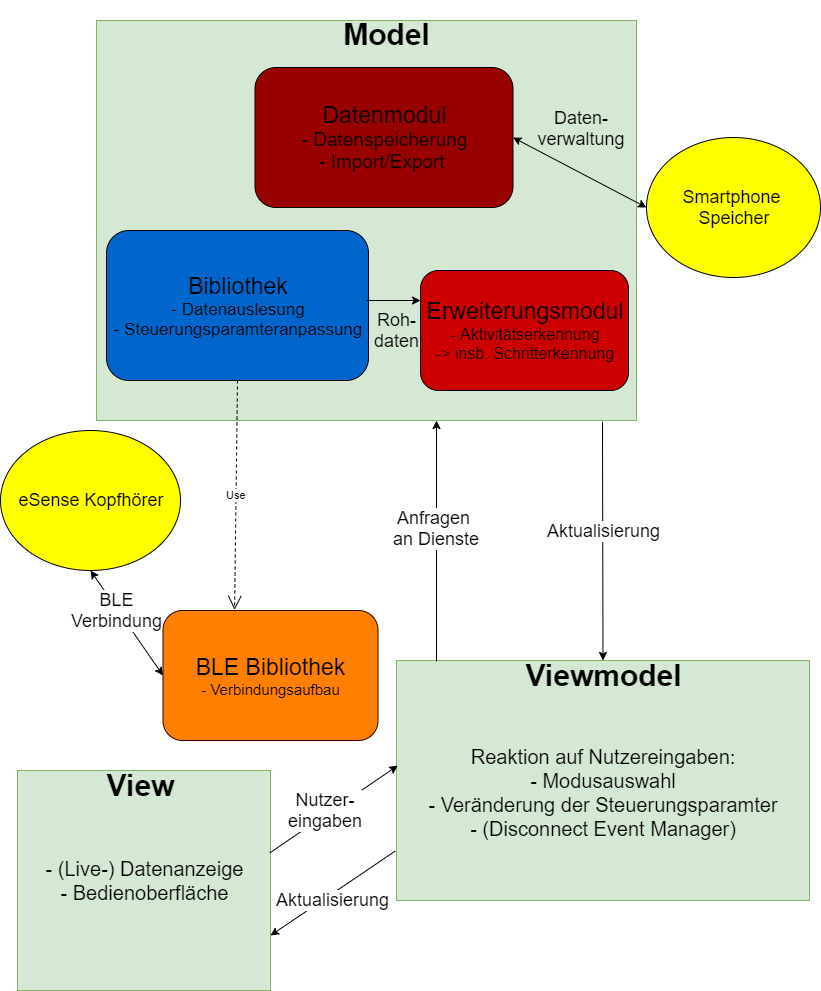
\includegraphics[width=0.8\textwidth]{./Diagramme/Achi5.png}
	\end{center}
	\clearpage %%sieht sonst noch zerrissener aus;    Gehts nicht irgendwie schöner? Sodass das Diagramm ganz oben quasi anliegt?
	\subsection{Kurze Erläuterung zum Architekturdiagramm}
  Wir haben uns bei der Architekturdiagramm für \textsf{Model-View-Viewmodel}, eine Spezialisierung  des Entwurfsmusters Model-View-Controller, entschieden.
  Dabei gibt es folgende Komponenten:
  \begin{itemize}
    \item \textsf{\glqq View\grqq{}} enthält alle grafisch angezeigten Elemente, also die Datenanzeige und Bedienoberfläche der App.
    \item {\textsf{\glqq Model\grqq{}} enthält die Geschäftslogik der App und ist stark nach außen abgekapselt. In diesen Bereich fallen die meisten komplexen Teile der App, die als Dienste (Services) vom Viewmodel aus verwaltet werden sollen. Wesentlich sind dabei (vollständige Angabe im Entwurf): \begin{itemize}
      \item Die Verwaltung der anfallenden Produktdaten (Abruf und Bereitstellung der gespeicherten Daten in der Datenbank, im CSV-Format) über ein Datenmodul
      \item Die Bibliothek, die für die Kommunikation mit den \Gls{Earables} (Verbindungsaufbau, Start und Stopp des Samplings, Konfiguration der \Gls{Steuerungsparameter}, Auslesen der Sensordaten) zuständig ist. Dazu wird eine externe Bibliothek\footnote{https://github.com/xabre/xamarin-bluetooth-le} verwendet.
      \item Das Erweiterungsmodul, das sich um die Aktivitätserkennung kümmert. Dieses nutzt dabei die Schnittstellen der Bibliothek.
    \end{itemize}
    Die Services sind dabei jeweils unabhängig vom restlichen Model funktionsfähig und dadurch leichter testbar.}
    \item \textsf{\glqq Viewmodel\grqq{}} ist das Bindeglied zwischen View und Model. Es enthält die Logik der UI, wird also bei Benutzerinteraktion vom View aufgerufen. Es gibt dann die entsprechenden Anweisungen an das Model weiter. Darüber hinaus kümmert es sich darum, dass in bestimmten Fällen die Anzeige der App angepasst wird, zum Beispiel bei Verbindungsabbruch zu den \Gls{Earables}. 
    
  \end{itemize}
  Der Vorteil dieser Architektur ist eine klare Trennung von Benutzerinteraktion und Programmlogik sowie eine lose Kopplung zwischen einzelnen Funktionalitäten, was die Flexibilität und das modulare Testen deutlich erleichtert.
\clearpage
  \subsection{Klassendiagramm}
hier kommt ein mal das Klassendiagramm rein mit Verweis auf den Anhang - valle
\clearpage
%%\section{Klassenübersicht} brauchen wir nicht, da das bei uns schon alles im Inhaltsverzeichnis aufgelistet wird.
\section{Klassenbeschreibung Model}
\subsection{Bibliothek}

\begin{minipage}[b]{0.3\textwidth}
	\subsubsection{Interface IEarablesConnection}
	
	\end{minipage}
	\begin{minipage}[c]{0.7\textwidth}
	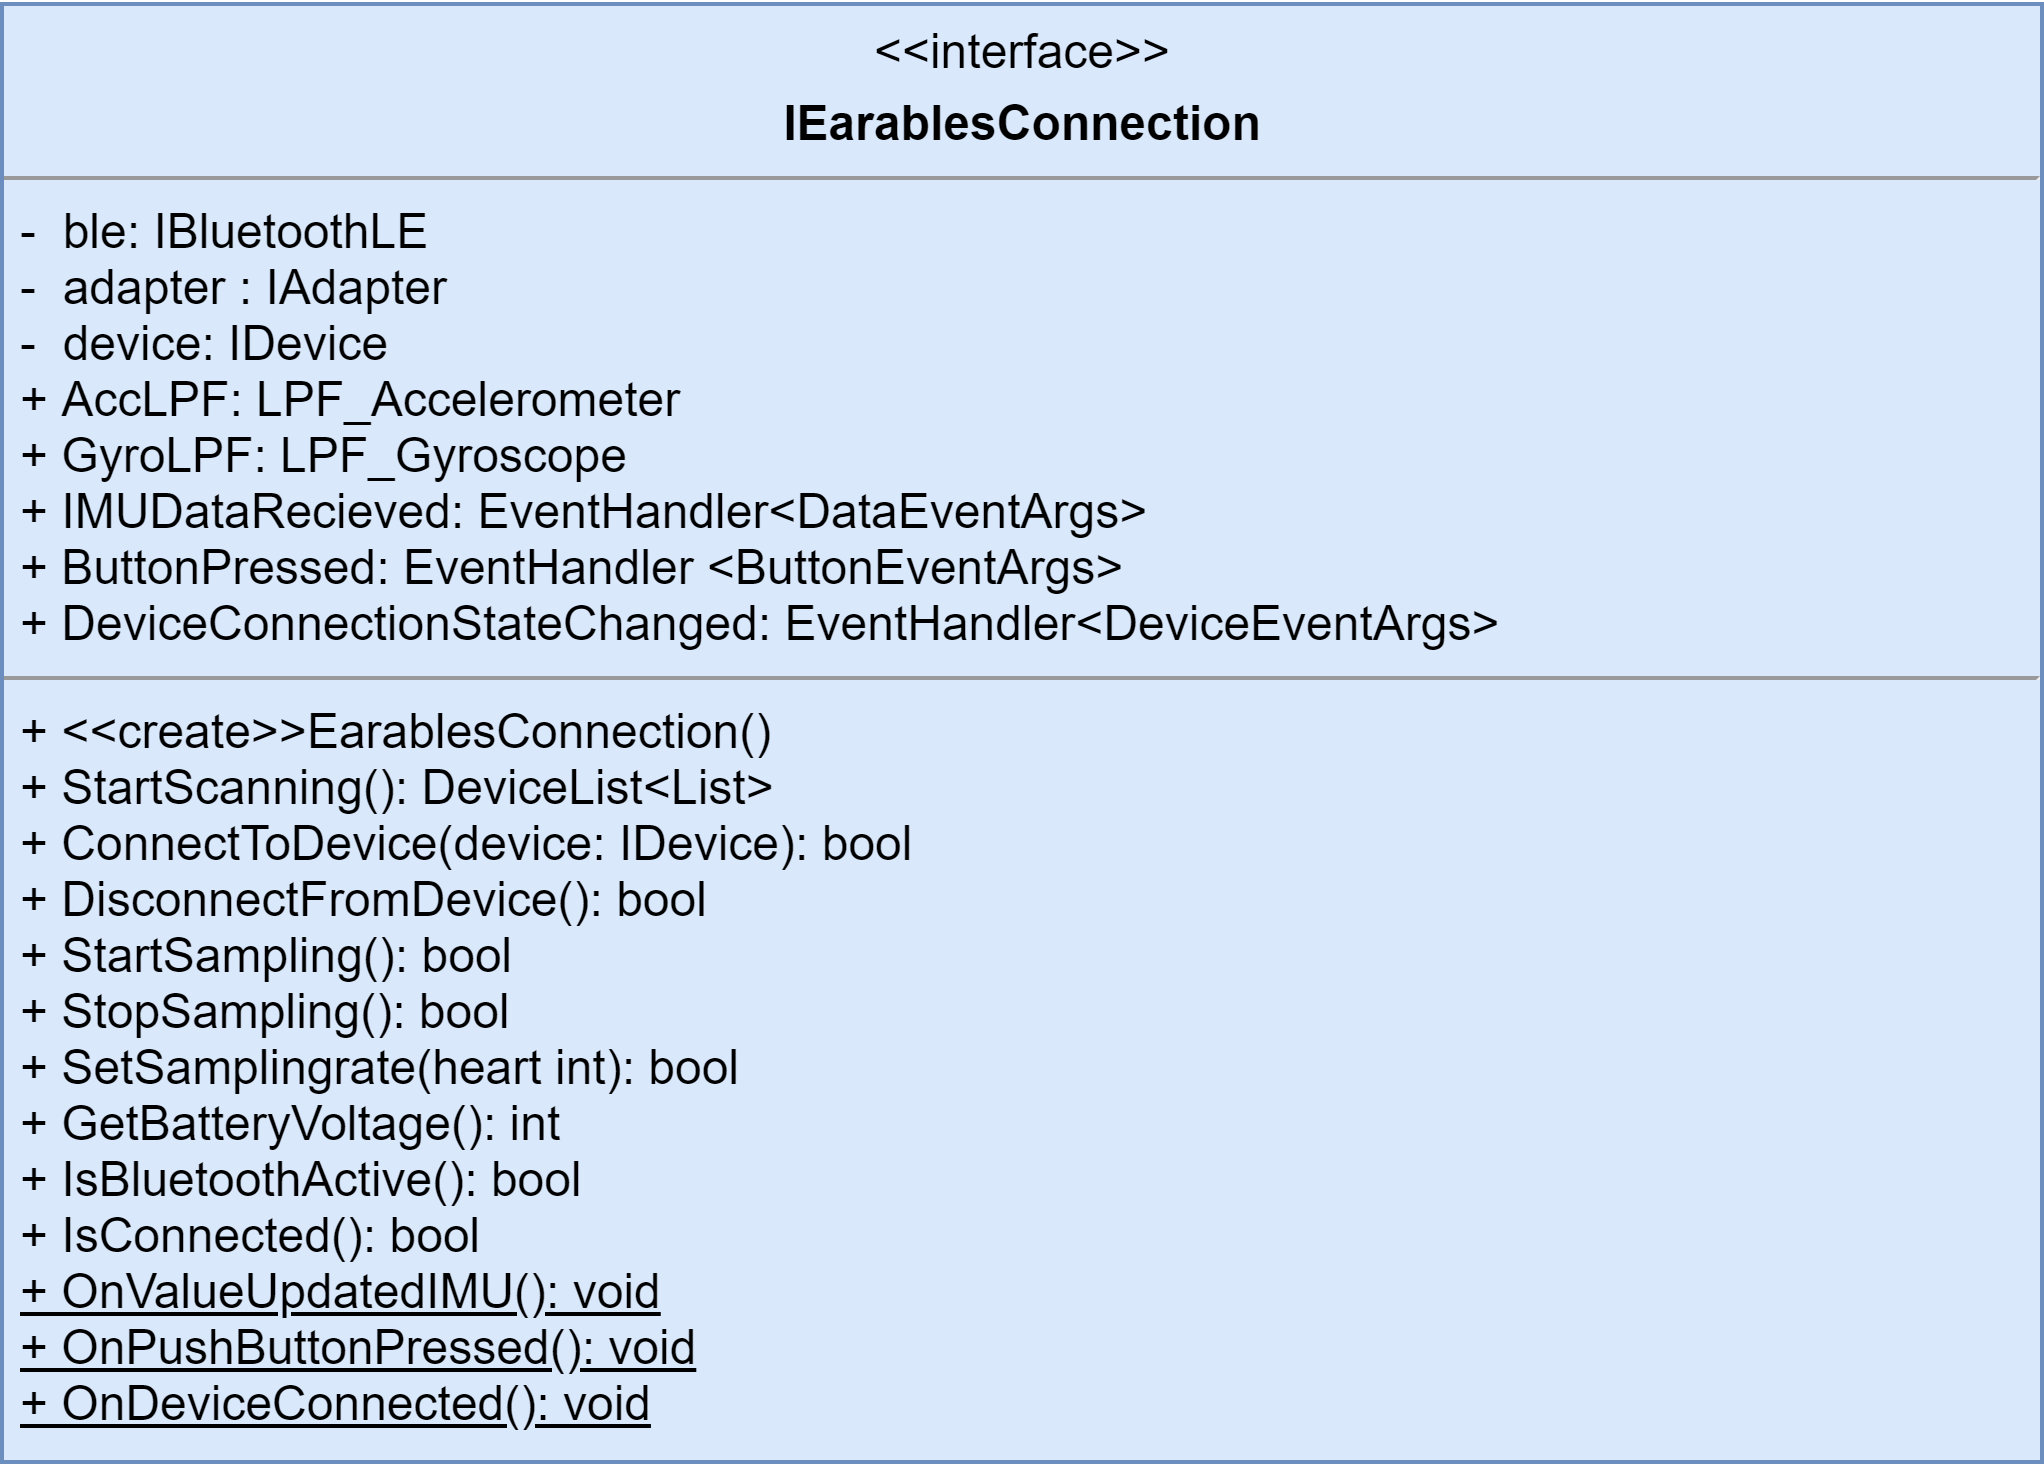
\includegraphics[width=1.5\textwidth]{bilder/BibPackageKlassen/IEarablesConnection.png}
\end{minipage}

\paragraph{Klassenbeschreibung:}
Diese Klasse ist das Herz der Bibliothek. Sie ist die Schnittstellen, über die später kommuniziert werden kann. Hierbei handelt es sich um ein Interface um Mocking zu ermöglichen und so das Implementieren und Testen zu vereinfachen. Um eine BLE Verbindung herzustellen benutzt sie das \glqq Bluetooth LE Plugin for Xamarin\grqq{}.

\paragraph{Attribute:}
\begin{itemize}
	\item[$-$] \textbf{ble: IBluetoothLE}\\ Wird benötigt um auf das Bluetooth des Smartphones zuzugreifen. Der Typ IBluetooth befindet sich im BLE\_Plugin
	\item[$-$] \textbf{adapter: IAdapter}\\ Wird benötigt um die Bluetoothverbindung aufzubauen. Der Typ  IAdapter befindet sich im BLE\_Plugin
	\item[$-$] \textbf{device: IDevice}\\ Wird benötigt um die Bluetoothverbindung aufzubauen. Der Typ  IDevice befindet sich im BLE\_Plugin
	\item[+] \textbf{IMUDataReceived: EventHandler<DataEventArgs>}\\Das Attribut IMUDataReceived beinhaltet die IMU Daten eines Eintrags und die Konfiguration der \Gls{Earables}.
	\item[+] \textbf{ButtonPressed: EventHandler <ButtonEventArgs>}\\ Das Attribut buttonPressed wird benötigt, um das Drücken des Knopfes an den \Gls{Earables} weiterleiten zu können.
	\item[+] \textbf{DeviceConnectionStateChanged: EventHandler<DeviceEventArgs>}\\ Das Attribut deviceConnectionStateChanged wird benötigt, um den aktuellen Verbindungsstatus weiterleiten zu können.
	\item[+] \textbf{Config: ConfigContainer}\\ In diesem Attribut befinden sich die Konfigurationsvariablen für die \Gls{Earables}.
	\item[+] \textbf{Characters: Characteristic}\\ Das Attribut enthält alle Charakteristiken die angesprochen werden müssen.
\end{itemize}
\paragraph{Methoden:}
\begin{itemize}
	\item[+] \textbf{<<create>>\Gls{Earables}Connection()}\\ Im Konstruktor werden die Attribute ble und adapter initialisiert.
	\item[+] \textbf{StartScanning(): DeviceList<List>}\\ Diese Methode legt eine neue Liste vom Typ IDevice an, in der sie alle gefundenen Devices speichert und anschließend zurückgibt. Sie benutzt die Methode DeviceDiscovered und StartScanningForDevicesAsync aus dem Interface IAdapter.
	\item[+] \textbf{ConnectToDevice(device: Idevice): bool}\\ Mit dieser Methode kann sich der Nutzer mit einem Bluetooth fähigen Gerät verbinden. Er wählt in der Liste  ein Device aus und übergibt es als Parameter. Falls die Verbindung erfolgreich war wird true zurückgegeben. Konnte keine Verbindung hergestellt werden wird false zurückgegeben. Hierbei wird die Methode ConnectToDeviceAsync aus dem BLE\_Pugin der Klasse IAdapter zur Hilfe genommen. Zusätzlich werden gleich alle benötigten Charakteristiken geladen und abgespeichert um sie nicht immer neu laden zu müssen, wenn sie gebraucht werden. Das geschieht mit Hilfe der Methoden GetServiceAsync und GetCharacteristicAsync aus dem BLE\_Plugin. Zum Schluss werden noch die Handler für die entsprechenden Events registriert und die Aktualisierung mit der Methode StartUpdatesAsync, aus dem BLE\_Plugin, gestartet.
	\item[+] \textbf{DisconnectFromDevice(): bool}\\ Falls man eine Verbindung zu einem Device besitzt wird diese getrennt und es wird true zurückgegeben. Wenn man keine Verbindung besitzt passiert nichts und es wird false zurückgegeben. Zum Trennen der Verbindung wird die Methode DisconnectDeviceAsync aus dem BLE\_Pugin der Klasse IAdapter benutzt.
	\item[+] \textbf{StartSampling(): bool}\\ Diese Methode startet die Datenaufzeichnung des IMU. Falls die Datenaufzeichnung erfolgreich gestartet wurde wird true zurückgegeben, ansonsten false. Die Methode WriteAsync aus dem BLE\_Plugin ermöglicht es die Charakteristik zu beschreiben. Hinweis: Ist die Samplingrate nicht gesetzt, wird die Standarteinstellung genommen.
	\item[+] \textbf{StopSampling(): bool}\\Die Datenaufzeichnung des IMU wird mit dieser Methode gestoppt. Falls die Datenaufzeichnung erfolgreich gestoppt wurde wird true zurückgegeben, ansonsten false. Die Methode WriteAsync aus dem BLE\_Plugin ermöglicht es die Charakteristik zu beschreiben.
	\item[+] \textbf{SetSamplingrate(heart int): booln}\\Die Samplingrate wird gesetzt und gespeichert. Bei erfolgreichem setzen wird true zurückgegeben ansonsten false. Die Methode WriteAsync aus dem BLE\_Plugin ermöglicht es die Charakteristik zu beschreiben.
	\item[+] \textbf{SetLowPassFilterAccelerometer(accelerometerLPF LPF\_Accelerometer): bool}\\ Im Konstruktor werden die Attribute ble und adapter initialisiert.
	\item[+] \textbf{GetLowPassFilterAccelerometer(): LPF\_Accelerometer}\\ Die Methode gibt an auf was der LPF des Accelerometers momentan gesetzt ist. Er wird in Form des LPF\_Accelerometer Enums zurückgegeben. 
	\item[+] \textbf{SetLowPassFilterGyroscope(gyroscopeLPF LPF\_Gyroscope): bool}\\ Mit dieser Methode wird der Low Pass Filter des Gyroskops gesetzt. Bei erfolgreichem setzen wird true zurückgegeben ansonsten false. Bei dem Übergabeparameter handelt es sich um ein Enum, der angibt auf welchen Wert der Low Pass Filter gesetzt werden soll. Die Methode WriteAsync aus dem BLE\_Plugin ermöglicht es die Charakteristik zu beschreiben.
	\item[+] \textbf{GetLowPassFilterGyroscope(): LPF\_Gyroscope}\\Die Methode gibt an auf was der LPF des Gyroskops momentan gesetzt ist. Er wird in Form des LPF\_Gyroscope Enums zurückgegeben. 
	\item[+] \textbf{GetBatteryVoltage(): int}\\ Gibt die Voltanzahl der Batterie zurück. Die Methode ReadAsync aus dem BLE\_Plugin ermöglicht es die entsprechende Charakteristik zu lesen.
	\item[+] \textbf{IsBluetoothActive(): bool}\\ Zeigt an ob Bluetooth auf dem Smartphone aktiviert ist. Gibt true zurück falls es aktiviert ist und false, falls nicht.
	\item[+] \textbf{static OnValueUpdatedIMU(): void}\\Falls neue IMU-Daten vorliegen, wird diese Methode aufgerufen und feuert das Event IMUDataRecieved.
	\item[+] \textbf{static OnPushButtonPressed(): void}\\ Falls der Knopf an den \Gls{Earables} gedrückt wurde, wird diese Methode aufgerufen und feuert das Event ButtonPressed: EventHandler.
	\item[+] \textbf{static OnDeviceConnected(): void}\\ Falls eine Verbindung mit einem Device hergestellt wurde oder eine bestehende Verbindung aufgelöst wurde, wird diese Methode aufgerufen und feuert das Event DeviceConnectionStateChanged.
\end{itemize}



\begin{minipage}[b]{0.5\textwidth}
	\subsubsection{Class EarablesConnection}
	
	\end{minipage}
	\begin{minipage}[c]{0.5\textwidth}
	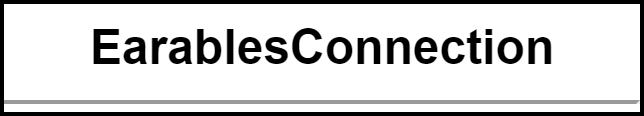
\includegraphics[width=0.8\textwidth]{bilder/BibPackageKlassen/EarablesConnection.png}
\end{minipage}

\paragraph{Klassenbeschreibung:}
Die Klasse EarablesConnection implementiert das IEarablesConnection Interface und ist die konkrete Klasse, die sich um die BLE-Verbindung kümmert.\\


\begin{minipage}[b]{0.5\textwidth}
	\subsubsection{Static Class Constants}
	
	\end{minipage}
	\begin{minipage}[c]{0.5\textwidth}
	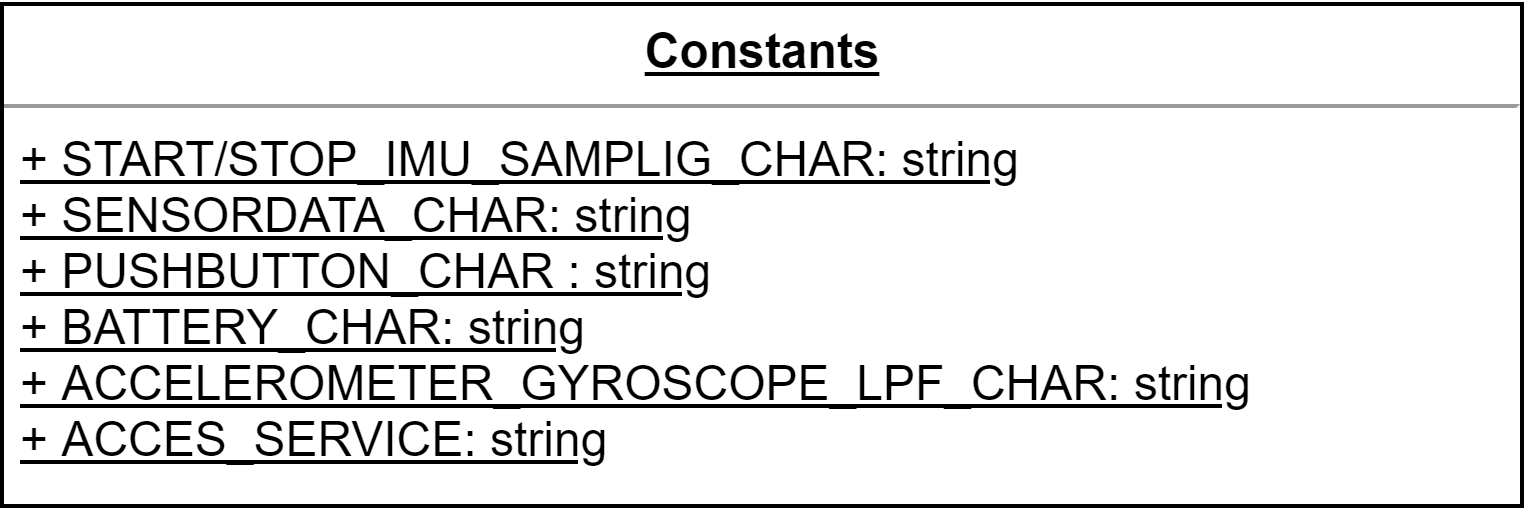
\includegraphics[width=1.4\textwidth]{bilder/BibPackageKlassen/Constants.png}
\end{minipage}

\paragraph{Klassenbeschreibung:}
Die Constants Klasse enthält alle Konstanten, die benötigt werden um die entsprechenden Service und Charakteristiken aus den \Gls{Earables} zu lesen. Sie ist als static gekennzeichnet da es keinen Sinn macht sie zu instanziieren, da sie nur Konstanten bereitstellt.

\paragraph{Attribute:}
\begin{itemize}
	\item[+] \textbf{START/STOP\_IMU\_SAMPLIG\_CHAR: String}\\Dieser String enthält die Beschreibung der Charakteristik um das IMU Daten Sampling zu starten und zu stoppen.
	\item[+] \textbf{SENSORDATA\_CHAR: String}\\Dieser String enthält die Beschreibung der Charakteristik in dem die IMU Sensordaten gespeichert werden.
	\item[+] \textbf{PUSHBUTTON\_CHAR: String}\\Dieser String enthält die Beschreibung der Charakteristik in dem der Push Button Status gespeichert wird.
	\item[+] \textbf{BATTERY\_CHAR: String}\\Dieser String enthält die Beschreibung der Charakteristik in dem die Batterieladung gespeichert wird.
	\item[+] \textbf{ACCELEROMETER\_GYROSCOPE\_LPF\_CHAR: String}\\Dieser String enthält die Beschreibung der Charakteristik in um den Low Pass Filter für den Accelerometer und das Gyroscope zu setzen.
\item[+] \textbf{ACCESS\_SERVICE: String}\\Dieser String enthält die Beschreibung des Services Access-Service, der die meisten Charakteristiken bereitstellt.
\end{itemize}


\begin{minipage}[b]{0.5\textwidth}
	\subsubsection{Class LPF\_Gyroscope}
	
	\end{minipage}
	\begin{minipage}[c]{0.5\textwidth}
	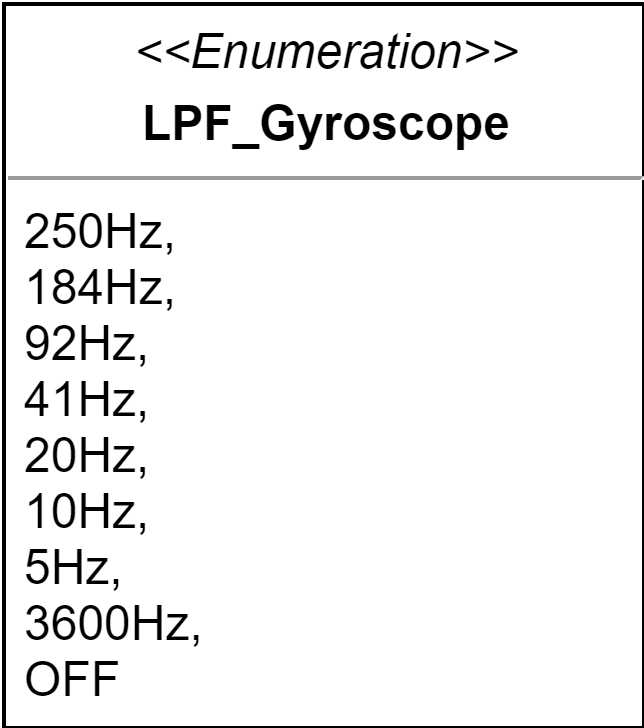
\includegraphics[width=0.8\textwidth]{bilder/BibPackageKlassen/LPF_Gyrosope.png}
\end{minipage}

\paragraph{Klassenbeschreibung:}
Dieses Enum beinhaltet alle möglichen Low Pass Filter Werte, die der LPF für das Gyroscope annehmen kann.

\paragraph{Attribute:}
\begin{itemize}
	\item \textbf{250Hz}\\Steht dafür, dass der LPF 250 Hz annehmen kann.
	\item \textbf{184Hz}\\Steht dafür, dass der LPF 184 Hz annehmen kann.
	\item \textbf{92Hz}\\Steht dafür, dass der LPF 92 Hz annehmen kann.
	\item \textbf{41Hz}\\Steht dafür, dass der LPF 41 Hz annehmen kann.
	\item \textbf{20Hz}\\Steht dafür, dass der LPF 20 Hz annehmen kann.
	\item \textbf{10Hz}\\Steht dafür, dass der LPF 10 Hz annehmen kann.
	\item \textbf{5Hz}\\Steht dafür, dass der LPF 5 Hz annehmen kann.
	\item \textbf{3600Hz}\\Steht dafür, dass der LPF 3600 Hz annehmen kann.
	\item \textbf{OFF}\\Steht dafür, dass der LPF aus ist.
\end{itemize}


\begin{minipage}[b]{0.5\textwidth}
	\subsubsection{Class LPF\_Accelerometer}
	
	\end{minipage}
	\begin{minipage}[c]{0.5\textwidth}
	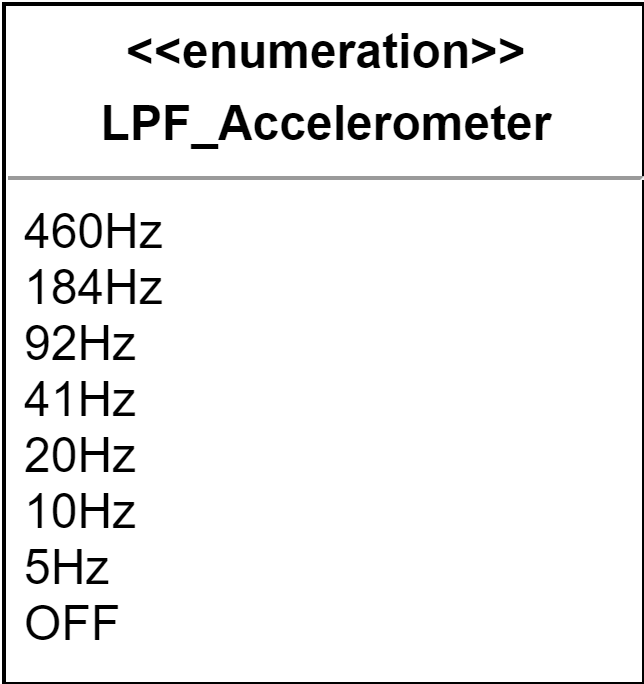
\includegraphics[width=0.8\textwidth]{bilder/BibPackageKlassen/LPF_Accelerometer.png}
\end{minipage}
\paragraph{Klassenbeschreibung:}
Dieses Enum beinhaltet alle möglichen Low Pass Filter Werte, die der LPF für das Accelerometer annehmen kann.

\paragraph{Attribute:}
\begin{itemize}
	\item \textbf{460Hz}\\Steht dafür, dass der LPF 460 Hz annehmen kann.
	\item \textbf{184Hz}\\Steht dafür, dass der LPF 184 Hz annehmen kann.
	\item \textbf{92Hz}\\Steht dafür, dass der LPF 92 Hz annehmen kann.
	\item \textbf{41Hz}\\Steht dafür, dass der LPF 41 Hz annehmen kann.
	\item \textbf{20Hz}\\Steht dafür, dass der LPF 20 Hz annehmen kann.
	\item \textbf{10Hz}\\Steht dafür, dass der LPF 10 Hz annehmen kann.
	\item \textbf{5Hz}\\Steht dafür, dass der LPF 5 Hz annehmen kann.
	\item \textbf{OFF}\\Steht dafür, dass der LPF aus ist.
\end{itemize}



\begin{minipage}[b]{0.5\textwidth}
	\subsubsection{Class ConfigContainer}
	
	\end{minipage}
	\begin{minipage}[c]{0.5\textwidth}
	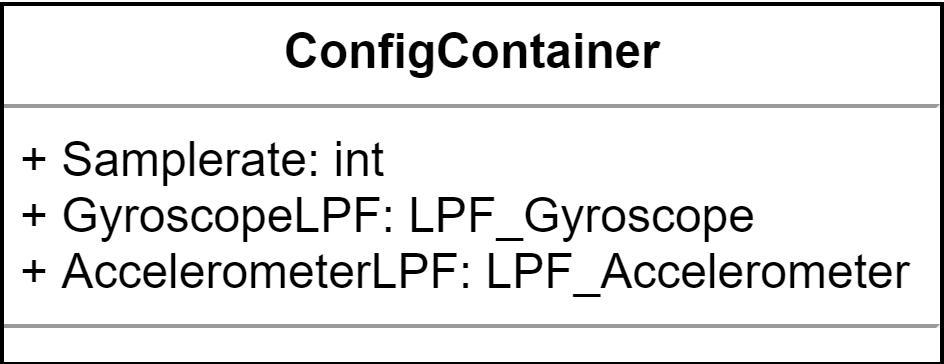
\includegraphics[width=0.8\textwidth]{bilder/BibPackageKlassen/ConfigContainer.png}
\end{minipage}
\paragraph{Klassenbeschreibung:}
Diese Klasse beinhaltet alle Einstellungsmöglichkeiten für die \Gls{Earables}.

\paragraph{Attribute:}
\begin{itemize}
	\item[+] \textbf{Samplerate: int}\\Hier wird die Samplerate gespeichert, in der die \Gls{Earables} neue Daten des IMU aufzeichnen.
	\item[+] \textbf{GyroscopeLPF: LPF\_Gyroscope}\\Dieses Attribut enthält den aktuell eingestellten LPF für das Gyroscope.
	\item[+] \textbf{AccelerometerLPF: LPF\_Accelerometer}\\Dieses Attribut enthält den aktuell eingestellten LPF für den Accelerometer.
\end{itemize}


\begin{minipage}[b]{0.5\textwidth}
	\subsubsection{Static Class IMUDataExtractor}
	
	\end{minipage}
	\begin{minipage}[c]{0.5\textwidth}
	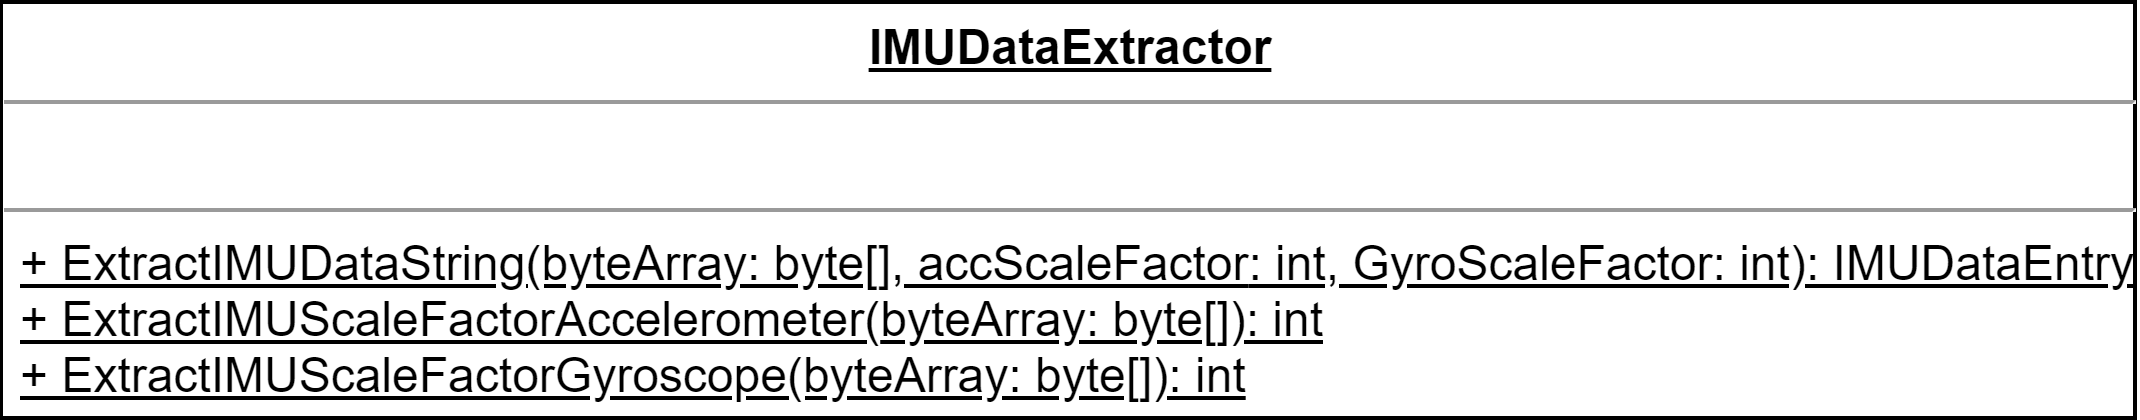
\includegraphics[width=0.8\textwidth]{bilder/BibPackageKlassen/IMUDataExtractor.png}
\end{minipage}
\paragraph{Klassenbeschreibung:}
Diese Klasse Übernimmt das Umwandeln des Bit Strings in vernünftige Werte und Einheiten.
Die Klasse wurde erstellt um dem IEarablesConnection Interface Arbeit abzunehmen und Logik zu entkoppeln, so dass sich das IEarablesConnection
Interface nur um die Kommunikation mit den \Gls{Earables} kümmern muss. Sie ist static da es keinen Sinn macht sie zu instanziieren, da sie nur einen Dienst anbietet.

\paragraph{Methoden:}
\begin{itemize}
	\item[+] \textbf{ExtractIMUDataString(byteString: int, accScaleFactor: int, GyroScaleFactor): IMUDataEntry}\\Diese Methode erstellt aus der übergebenen Bitfolge ein IMUDataEntry, indem sie die Informationen aus dem Bit String auswertet und in verschiedene Einheiten umrechnet. Zum umrechnen benötigt sie noch den accScaleFactor und den gyroScaleFactor. Sie erzeugt ein neues IMUDataEntry Objekt und gibt es als Rückgabewert zurück.
\end{itemize}


\begin{minipage}[b]{0.5\textwidth}
	\subsubsection{Class IMUDataEntry}
	
	\end{minipage}
	\begin{minipage}[c]{0.5\textwidth}
	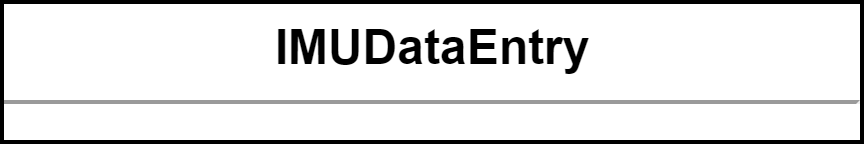
\includegraphics[width=0.8\textwidth]{bilder/BibPackageKlassen/IMUDataEntry.png}
\end{minipage}
\paragraph{Klassenbeschreibung:}
Diese Klasse besitzt alle ausgewerteten Informationen, die in einem „Packet“ von den \Gls{Earables} ankommen.

\paragraph{Attribute:}
\begin{itemize}
	\item[+] \textbf{Gyro: Gyroscope}\\In diesem Attribut sind die gemessenen Werte des Gyroscopes enthalten.
	\item[+] \textbf{Acc: Accelerometer}\\In diesem Attribut sind die gemessenen Werte des Accelerometers enthalten.
\end{itemize}




\begin{minipage}[b]{0.5\textwidth}
	\subsubsection{Class Gyroscope}
	
	\end{minipage}
	\begin{minipage}[c]{0.5\textwidth}
	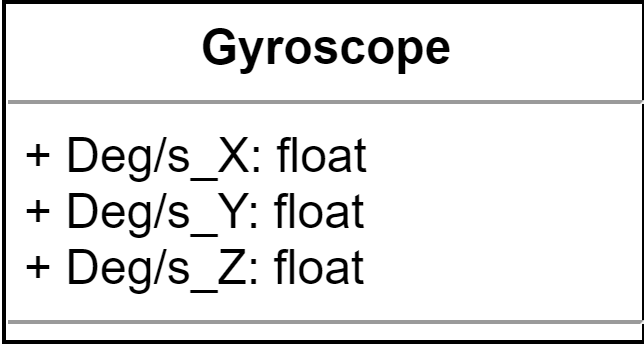
\includegraphics[width=0.8\textwidth]{bilder/BibPackageKlassen/Gyroscope.png}
\end{minipage}
\paragraph{Klassenbeschreibung:}
Diese Klasse besitzt alle ausgewerteten Gyroskopdaten.

\paragraph{Attribute:}
\begin{itemize}
	\item[+] \textbf{Deg/s\_X: float}\\Gibt an um wie viel Grad pro Sekunde sie die \Gls{Earables} in X Richtung gedreht haben.
	\item[+] \textbf{Deg/s\_Y: float}\\Gibt an um wie viel Grad pro Sekunde sie die \Gls{Earables} in Y Richtung gedreht haben.
	\item[+] \textbf{Deg/s\_Z: float}\\Gibt an um wie viel Grad pro Sekunde sie die \Gls{Earables} in Z Richtung gedreht haben.
\end{itemize}


\begin{minipage}[b]{0.5\textwidth}
	\subsubsection{Class Accelerometere}
	
	\end{minipage}
	\begin{minipage}[c]{0.5\textwidth}
	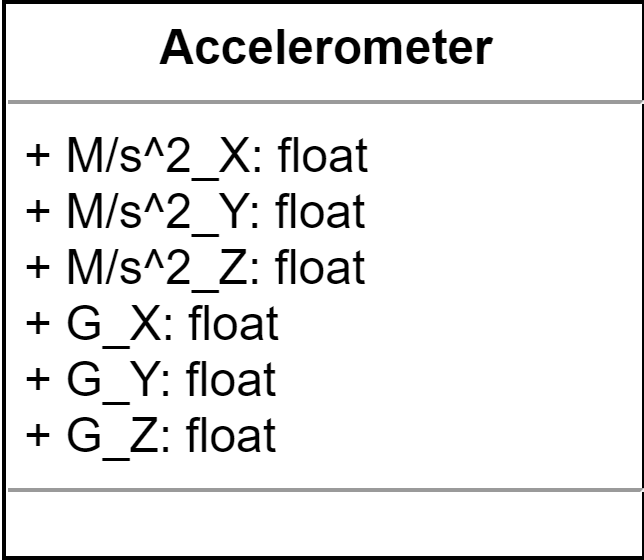
\includegraphics[width=0.8\textwidth]{bilder/BibPackageKlassen/Accelerometer.png}
\end{minipage}
\paragraph{Klassenbeschreibung:}
Diese Klasse besitzt alle ausgewerteten Accelerometer Daten.

\paragraph{Attribute:}
\begin{itemize}
	\item[+] \textbf{M/s$^2$\_X: float}\\Gibt an um wie viel $m/s^2$ sich die \Gls{Earables} in X Richtung beschleunigt haben.
	\item[+] \textbf{M/s$^2$\_Y: float}\\Gibt an um wie viel $m/s^2$ sich die \Gls{Earables} in Y Richtung beschleunigt haben.
	\item[+] \textbf{M/s$^2$\_Z: float}\\Gibt an um wie viel $m/s^2$ sich die \Gls{Earables} in Z Richtung beschleunigt haben.
	\item[+] \textbf{G\_X: float}\\Gibt an um wie viel G sich die \Gls{Earables} in X Richtung beschleunigt haben.
	\item[+] \textbf{G\_Y: float}\\Gibt an um wie viel G sich die \Gls{Earables} in Y Richtung beschleunigt haben.
	\item[+] \textbf{G\_Z: float}\\Gibt an um wie viel G sich die \Gls{Earables} in Z Richtung beschleunigt haben.
\end{itemize}



\begin{minipage}[b]{0.5\textwidth}
	\subsubsection{Class Characteristics}
	
	\end{minipage}
	\begin{minipage}[c]{0.5\textwidth}
	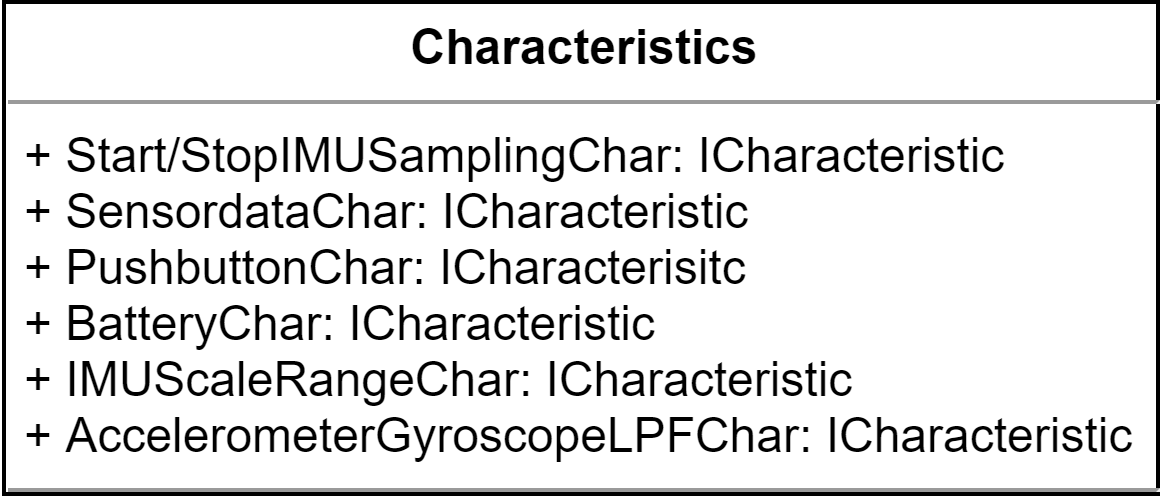
\includegraphics[width=0.8\textwidth]{bilder/BibPackageKlassen/Characteristics.png}
\end{minipage}
\paragraph{Klassenbeschreibung:}
In dieser Klasse werden die Charakteristiken gespeichert um sie nicht jedes mal neu zu laden wenn sie gebraucht werden. Der Datentyp ICharacteristic befindet sich in dem BLE-Plugin.

\paragraph{Attribute:}
\begin{itemize}
	\item[+] \textbf{Start/StopIMUSamplingChar: ICharacteristic}\\Speichert die Charakteristik um das IMU sampling zu starten oder zu stoppen.
	\item[+] \textbf{Sensordata: ICharacteristicChar}\\Speichert die Charakteristik in der die Sensordaten liegen.
	\item[+] \textbf{Pushbutton: ICharacteristicChar}\\Speichert die Charakteristik in der der Status des Push Button gespeichert wird.
	\item[+] \textbf{Battery: ICharacteristicChar}\\Speichert die Charakteristik in der die verbleibende Battrieladung gespeichert wird.
	\item[+] \textbf{AccelerometerGyroscopeLPFChar: ICharacteristic}\\Speichert die Charakteristik in der die Konfiguration des LPF für den Accelerometer und das Gyroscope geschrieben wird.
\end{itemize}


\begin{minipage}[b]{0.5\textwidth}
	\subsubsection{Class DeviceEventArgs}
	
	\end{minipage}
	\begin{minipage}[c]{0.5\textwidth}
	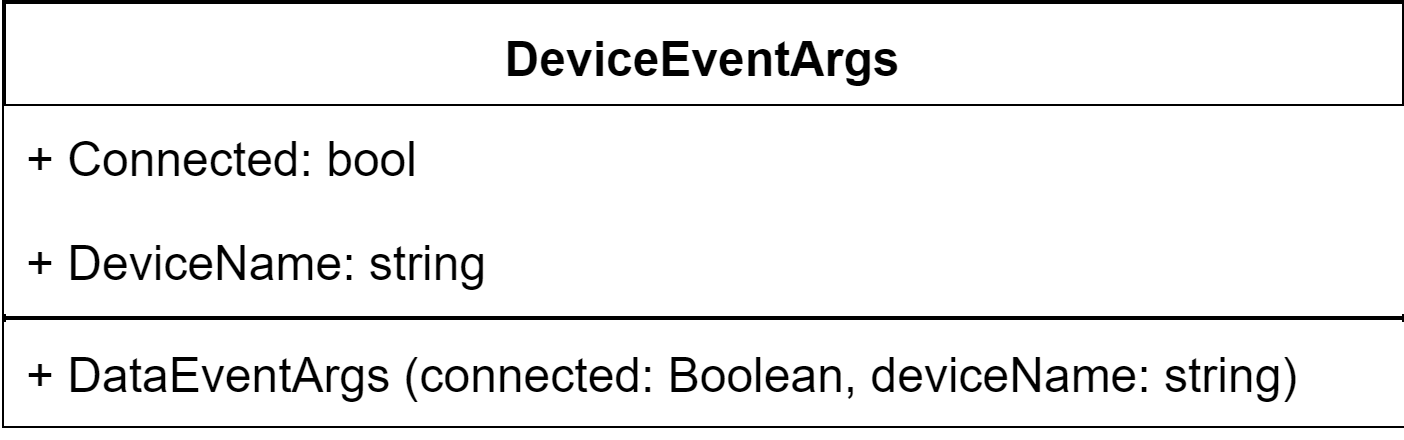
\includegraphics[width=0.8\textwidth]{bilder/BibPackageKlassen/DeviceEventArgs.png}
\end{minipage}
\paragraph{Klassenbeschreibung:}
Enthält alle relevanten Informationen, die als Parameter mit dem Event DeviceConnectionStateChanged gefeuert werden.

\paragraph{Attribute:}
\begin{itemize}
	\item[+] \textbf{Connected: bool}\\Ist true falls eine BLE Verbindung mit einem Device existiert und false falls nicht.
	\item[+] \textbf{DeviceName: String}\\Beinhaltet den Gerätenamen des Geräts, mit dem der Nutzer verbunden ist. 
\end{itemize}

\paragraph{Methoden:}
\begin{itemize}
	\item[+] \textbf{<<create>>DeviceEventArgs(connected: Boolean, deviceName: String): void}\\ Zusätzlicher Konstruktor um die Attribute setzten zu können
\end{itemize}


\begin{minipage}[b]{0.5\textwidth}
	\subsubsection{Class ButtonEventArgs}
	
	\end{minipage}
	\begin{minipage}[c]{0.5\textwidth}
	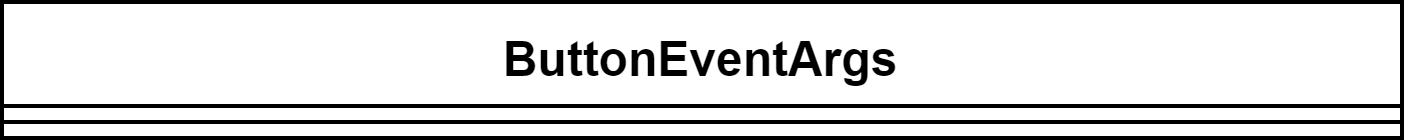
\includegraphics[width=0.8\textwidth]{bilder/BibPackageKlassen/ButtonEventArgs.png}
\end{minipage}
\paragraph{Klassenbeschreibung:}
Enthält alle relevanten Informationen, die als Parameter mit dem Event ButtonPressed gefeuert werden. Momentan ist diese Klasse leer, aber sie existiert bereits falls bei der Weiterentwicklung des Moduls doch Argumente übergeben werden müssen.



\begin{minipage}[b]{0.5\textwidth}
	\subsubsection{Class DataEventArgs}
	
	\end{minipage}
	\begin{minipage}[c]{0.5\textwidth}
	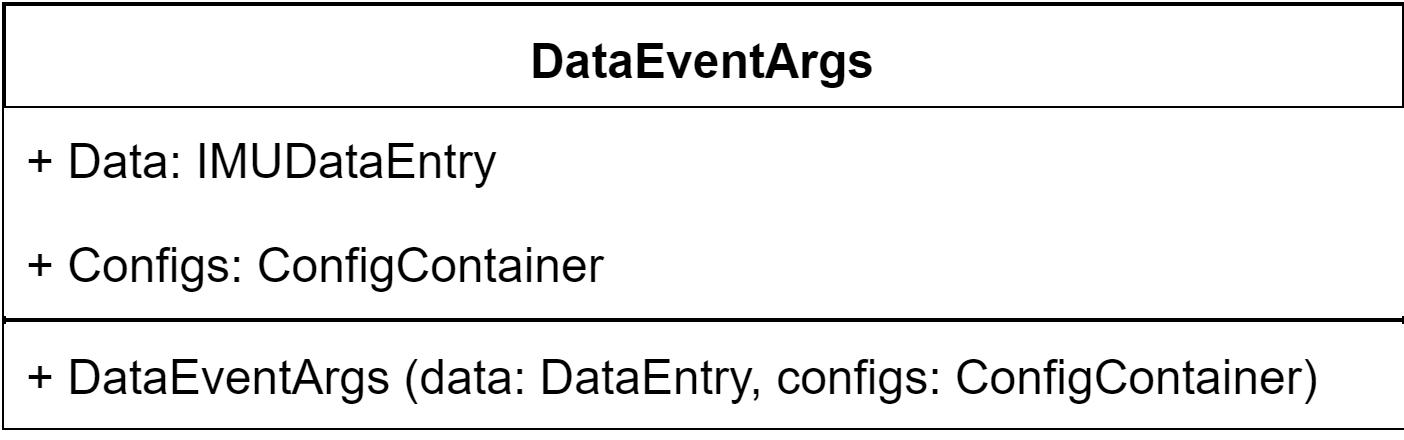
\includegraphics[width=0.8\textwidth]{bilder/BibPackageKlassen/DataEventArgs.png}
\end{minipage}
\paragraph{Klassenbeschreibung:}
Enthält alle relevanten Informationen, die als Parameter mit dem Event IMUDataRecieved gefeuert werden.

\paragraph{Attribute:}
\begin{itemize}
	\item[+] \textbf{Data: IMUDataEntry}\\Hier handelt es sich um die aktuellen IMU Datenaufzeichnung.
	\item[+] \textbf{Configs: ConfigContainer}\\Hier werden die aktuellen Konfigurationen gespeichert.
\end{itemize}

\paragraph{Methoden:}
\begin{itemize}
	\item[+] \textbf{<<create>>DataEventArgs(connected: bool, deviceName: String): void}\\ Zusätzlicher Konstruktor um die Attribute setzten zu können
\end{itemize}






\subsection{Erweiterungsmodul}
\begin{center}
	\centering
	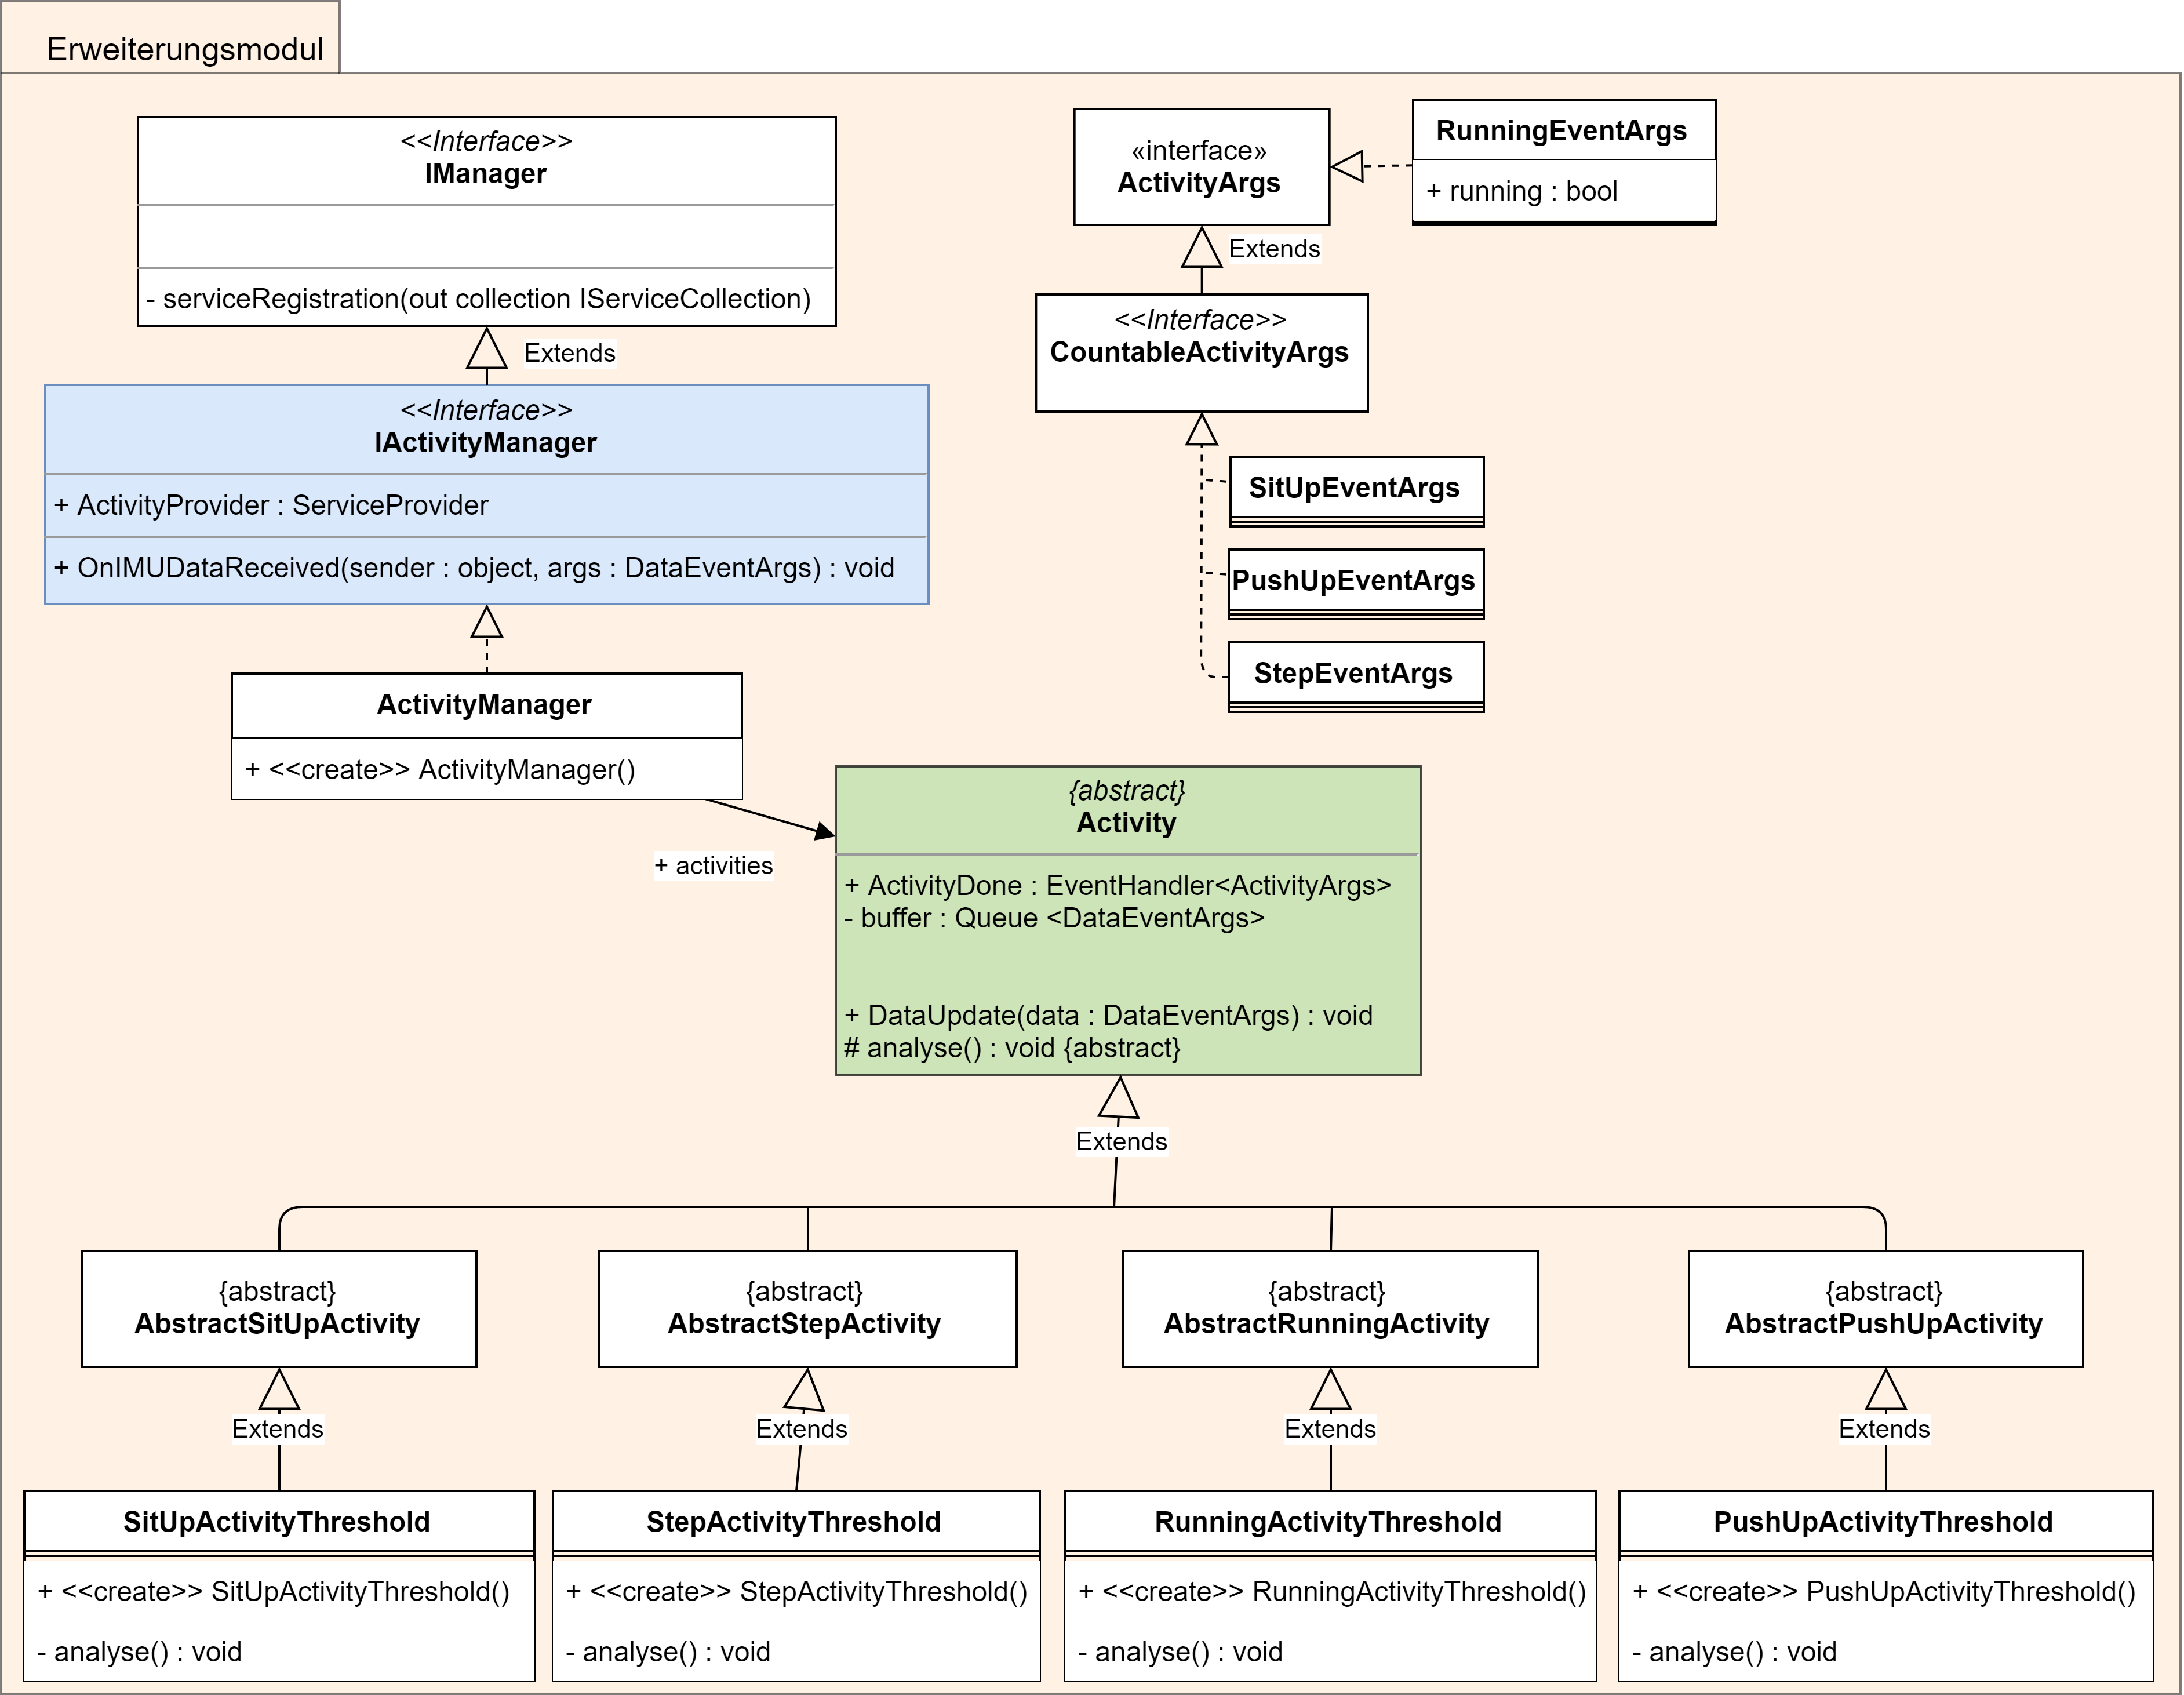
\includegraphics[width=15cm]{bilder/ErweiterungsmodulTest.png}
\end{center}

\begin{minipage}[b]{0.5\textwidth}
	\subsubsection{Interface IManager}
	
	\end{minipage}
	\begin{minipage}[c]{0.5\textwidth}
	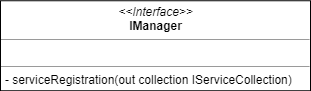
\includegraphics[width=\textwidth]{bilder/IManager.png}
\end{minipage}


	\paragraph{Schnittstellenbeschreibung:}
	Die Schnittstelle IManager definiert einen Service-Manager, welcher eine Menge an Services verwaltet. Dabei definiert die Schnittstelle die private Methode ServiceRegistration(out collection: IServiceCollection), um die Services bei der Erstanlegung zu registrieren. Diese muss bei einer Nutzung implementiert werden. Dabei implementieren zwei Komponenten die Schnittstelle IManager. (IActivityManager, ServiceManager). Die IServiceCollection ist aus der Erweiterung \Gls{DependencyInjection}
	
	\paragraph{Methoden:}
	\begin{itemize}
		\item[$-$] \textbf{ServiceRegistration(out collection: IServiceCollection)}\\Private Methode, welche eine IServiceCollection anlegt und die Services dort registriert. Die IServiceCollection wird zurückgegeben. 
	\end{itemize}
	
	\subsubsection{Interface IActivityManager}
	\paragraph{Schnittstellenbeschreibung:}
	Die Schnittstelle IActivityManager erweitert die Schnittstelle IManager. Dabei definiert IActivityManager einen spezielleren Service-Manager. Dieser beinhaltet die Modi Services. Zudem definiert der IActivityManager die EventMethode OnIMUDataReceived(sender: object, args: DataEventArgs).\\
	Die Schnittstelle ist bei der Klasse ServiceManager als Service registriert und kann über diese von anderen Komponenten in der App angesprochen werden.
	
	\paragraph{Attribute:}
	\begin{itemize}
		\item[+] \textbf{ActivityProvider: ServiceProvider}\\Das Attribut ActivityProvider ist vom Typ ServiceProvider, eine Klasse aus der Erweiterung \Gls{DependencyInjection}. Dabei sind in dieser die registrierten Services gespeichert. Über die Methode GetService<T>() bekommt man eine konkrete Instanz des Services vom Typ T zurück. 
	\end{itemize}
	
	\paragraph{Methoden:}
	\begin{itemize}
		\item[$-$] \textbf{ServiceRegistration(out collection IServiceCollection)}\\Die Methode wird von der Schnittstelle IManager geerbt. Diese wird benötigt, um einen ServiceProvider zu erstellen (hier für das Attribut ActivityProvider).
		\item[+] \textbf{OnIMUDataReceived(sender: object, args: DataEventArgs): void}\\Die öffentliche Methode ist eine EventMethode, welche beim EventHandler IMUDataReceived der Klasse EarablesConnection registriert wird. Die konkreten Unterklassen müssen diese implementieren. 
	\end{itemize}
	
	\subsubsection{Class ActivityManager}
	\paragraph{Klassenbeschreibung:}
	Die Klasse ActivityManager implementiert die Schnittstelle IActivityManager. Sie ist demnach ein Service-Manager und verwaltet die Activities (Vorgängeanalysen). Über sie können die ViewModels auf die Activities zugreifen.\\
	Der AktivityManager besitzt einen Service von den folgenden Typen: AbstractSitUpActivity, AbstractStepActivity, AbstractRunningActivity, AbstractPushUpActivity.\\
	Diese werden als Singletons gespeichert, was bedeutet, dass bei einem Aufruf von GetService<IT,T> immer die gleiche Instanz von T zurückgeliefert wird.
	
	\paragraph{Attribute:}
	\begin{itemize}
		\item[+] \textbf{activities: List<Activity>}\\Es wird eine Liste der registrierten Aktivitäten gespeichert. Bei einer Datenweitergabe muss somit nicht jedes mal vom ActivityProvider die Anfrage kommen, wer registriert ist. 
		\item[+] \textbf{ActivityProvider: ServiceProvider}\\Das Attribut beinhaltet die einzelnen Services mithilfe eines Dictionaries. Wird in dem Konstruktor instanziiert.
	\end{itemize}
	\paragraph{Methoden:}
	\begin{itemize}
		\item[+] \textbf{<<create>> ActivityManager}\\Hier handelt es sich um den Konstruktor der Klasse ActivityManager. In dieser wird sich bei dem EventHandler IMUDataReceived der Klasse EarablesConnection registriert und die private Methode ServiceRegistration(...) aufgerufen. Damit findet die Registrierung der Services und die Instanziierung des ActivityProviders statt.
		\item[$-$] \textbf{ServiceRegistration(out collection IServiceCollection): void}\\Private geerbte Methode der Schnittstelle IManager. In dieser wird eine ServiceCollection angelegt, bei der die Aktiväten registriert werden. Dabei passtiert dies mit der Methode collection.AddSingleton<IT,T>(). IT ist eine Oberklasse/Schnittstelle und T die konkrete Implementierung. IT ist in der Klasse ActivityManager immer vom Typ Activity (abstract).
		\item[+] \textbf{OnIMUDataReceived(sender: object, args: DataEventArgs): void}\\EventMethode, welche bei dem EventHandler IMUDataReceived der Klasse EarablesConnection registriert wird. Bei dem Aufrufen der Methode werden die Daten an die gespeicherten Aktivitäten weitergegeben. Das passiert per Push-Model (Observer-Muster). Bei den Aktivitäten wir die Methode DataUpdate(data: DataEventArgs) aufgerufen mit den bekommenen Daten als Parameter.
	\end{itemize}
	
	
	\subsubsection{Class Activity}
	\paragraph{Klassenbeschreibung}
	Activity ist eine abstrakte Klasse. Eine Activity ist im Wesentlichen ein Aktivitätserkennungsalgorithmus. Dabei wird die DataUpdate() Methode implementiert und den Unterklassen zu Verfügung gestellt. Der Algorithmus zur Aktivitätsanalyse (protected abstract void Analyse()) wird nur in konkreten Unterklassen implementiert, was in dem Entwurfsmuster der primitiven Operation entspricht.
	
	\paragraph{Attribute:}
	\begin{itemize}
		\item[+] \textbf{ActivityDone: EventHandler<ActivityArgs>}\\Bei dem EventHandler können sich die ViewModel registrieren. Diese werden benachrichtigt, wenn eine Aktivität durchgeführt wurde (Schritt gelaufen, Liegestütze gemacht, etc.). Der EventHandler wird in der Methode Analyse() aufgerufen. Als Argument bei der Eventwurf wird ein Objekt des Types ActivityArgs übergeben.
		\item [$-$] \textbf{buffer: Queue <DataEventArgs>}\\In der Queue werden die ankommenden Dateneinträge gespeichert. Diese werden nach einander von dem Algorithmus in Analyse() verwendet. 
	\end{itemize}
	\paragraph{Methoden:}
	\begin{itemize}
		\item[+] \textbf{DataUpdate(data: DataEventArgs): void}\\Mit dieser Methode bekommt die Aktivität die neuen Dateneinträge. Dabei ruft die Klasse ActivityManager die Methode auf, wenn sie die neuen Daten bekommt. In dieser Methode wird geschaut, ob sich ein Event bei dem EventHandler ActivityDone registriert hat. Falls ja, wird der Datensatz dem buffer hinugefügt, und der Algorithmus gestartet. Falls nicht, wird der Datensatz ignoriert.
		\item[\#] \textbf{abstract Analyse(): void}\\Der Algorithmus der Aktivitätserkennung wird in dieser Methode ausgeführt. Dabei ist dieser in den Unterklassen implementiert. Er beurteilt nur mithilfe der gesammelten Gyroskop- und Accelerometerdaten, ob das (der Activity entsprechende) Ereignis eingetroffen ist. In diesem Fall feuert er ein Event über den ActivityDone EventHandler. 
	\end{itemize}
	\subsubsection{Abstract class AbstractStepActivity}
	\paragraph{Klassenbeschreibung:}
	Diese Klasse dient nur zur Gewährleistung der Modularität für den ServiceManager. Alle Kinder dieser Klasse sind verschiedene Algorithmen zur Schritterkennung.\\ Es soll immer ein Event gefeuert werden, wenn ein Schritt getätigt wurde.
	\subsubsection{Class StepActivityActivityThreshold}
	\paragraph{Klassenbeschreibung:}
	Diese Klasse beinhaltet den Threshold-Algorithmus für die Erkennung, wann ein Schritt getätigt wurde. Es handelt sich hierbei um eine Kindklasse der abstrakten Klasse AbstractStepActivity. 
	\paragraph{Methoden:}
	\begin{itemize}
		\item [+]\textbf{<<create>> StepActivityThreshold(): void}\\Konstruktor der KlasseStepActivityThreshold. Dabei wird der EventHandler ActivityDone initialisiert. 
		\item [$-$]\textbf{Analyse(): void}\\ Implementierung der Analyse für die Schritterkennung. Dabei basiert diese auf dem Threshold Ansatz.  
	\end{itemize}
	
	\subsubsection{Abstract class AbstractRunningActivity}
	\paragraph{Klassenbeschreibung:}
	Diese Klasse dient nur zur Gewährleistung der Modularität für den ServiceManager. Alle Kinder dieser Klasse sind verschiedene Algorithmen zur Erkennung, ob der Nutzer läuft oder steht.\\ Es wird immer dann ein Event gefeuert, wenn sich dieser Status ändert.
	
	\subsubsection{Class RunningActivityThreshold}
	\paragraph{Klassenbeschreibung:}
	Diese Klasse beinhaltet den Threshold-Algorithmus für die Erkennung, ob der Nutzer läuft oder steht. Es wird nur analysiert, falls sich mindestens ein Event bei dem geerbten EventHandler ActivityDone registriert hat.
	\paragraph{Methoden:}
	\begin{itemize}
		\item [+]\textbf{<<create>> SitUpActivityThreshold(): void}\\Konstruktor der Klasse RunningActivityThreshold. In diesem wird der EventHandler erstellt.
		\item [$-$]\textbf{Analyse(): void}\\Implementierung der Analyse, ob der Nutzter läuft oder steht. Der EventHandler ActivityDone ruft die Events auf, falls sich der Laufstatus ändert. Das bedeutet, wenn der Nutzer anfängt zu laufen, oder aufhört. 
	\end{itemize}
	
	
	\subsubsection{Abstract class AbstractPushUpActivity}
	\paragraph{Klassenbeschreibung:}
	Diese Klasse dient nur zur Gewährleistung der Modularität für den ServiceManager. Alle Kinder dieser Klasse sind verschiedene Algorithmen zur Erkennung von Push-ups.\\ Es soll immer ein Event gefeuert werden, wenn eine Liegestütze erkannt wurde.
	
	\subsubsection{Class PushUpActivityThreshold}
	\paragraph{Klassenbeschreibung:}
	Diese Klasse beinhaltet den Threshold-Algorithmus für die Erkennung von Sit-ups.Es wird nur analysiert, falls sich mindestens ein Event bei dem geerbten EventHandler ActivityDone registriert hat.
	\paragraph{Methoden:}
	\begin{itemize}
		\item [+]\textbf{<<create>> PushUpActivityThreshold(): void}\\Konstruktor der Klasse PushUpActicityThreshold(). In diesem wird der EventHandler ActivityDone instanziiert. 
		\item [$-$]\textbf{Analyse(): void}\\Implementierung der Analyse für die Sit-Up-Erkennung. Dabei werden die Daten aus der Queue Buffer benutzt. Der EventHandler ruft die Events auf, wenn eine Liegestütze gemacht wurde.
	\end{itemize}

	\subsubsection{Abstract class AbstractSitUpActivity}
	\paragraph{Klassenbeschreibung:}
	Diese Klasse dient nur zur Gewährleistung der Modularität für den ServiceManager. Alle Kinder dieser Klasse sind verschiedene Algorithmen zur Erkennung von Sit-ups.\\ Es soll nach jedem erkannten Sit-up ein Event gefeuert werden.
	
	\subsubsection{Class SitUpActivityThreshold}
	\paragraph{Klassenbeschreibung:}
	Diese Klasse beinhaltet den Threshold-Algorithmus für die Erkennung von Sit-ups. Hier wird basierend auf den Daten der Earables der Algorithmus in der Methode Analyse() ausgeführt.
	\paragraph{Methoden:}
	\begin{itemize}
		\item [+]\textbf{<<create>> SitUpActivityThreshold(): void}\\Konstruktor der Klasse SitUpActivityThreshold. In dieser wird der EventHandler instanziiert. 
		\item [$-$]\textbf{Analyse(): void}\\ Implementierung der Analyse des Ereignisses. Dabei basiert dieser auf einem Threshold Ansatz. Diese wird nur ausgeführt, falls sich ein Event bei ActivityDone registriert hat.
	\end{itemize}
		
	
	\subsubsection{Interface ActivityArgs}
	\paragraph{Schnittstellenbeschreibung:}
	ActivityArgs werden beim Feuern eines Events mit dem Event übergeben. Das erkannte Ereignis kann durch die ActivityArgs genauer beschrieben werden. Dabei handelt es sich hierbei um eine Schnittstelle. 
	
	\subsubsection{Class RunningEventArgs}
	\paragraph{Klassenbeschreibung:}
	Ein Event der RunningActivityThreshold sagt entweder aus, dass der Nutzer stoppt, oder, dass er zu laufen beginnt.
	\paragraph{Attribute:}
	\begin{itemize}
		\item[+] \textbf{running: bool}\\ Dieses Attribut ist genau dann auf wahr (true) gesetzt, wenn der Nutzer zu laufen beginnt; falsch (false), wenn der Nutzer stoppt.
	\end{itemize} 

	\subsubsection{Interface CountableActivityArgs}
	\paragraph{Schnittstellenbeschreibung:}
	Diese Schnittstelle spezifiziert alle EventArgs bei Aktivitäten, bei denen gezählt werden kann. Auch wenn momentan keine weiteren EventArgs verwendet werden stärkt diese Struktur die Erweiterbarkeit und Übersichtlichkeit. Falls für zählbare Aktivitäten weitere Argumente angegeben werden sollen, kann dies gebündelt geschehen.
	
	\subsubsection{Class PushUpEventArgs}
	Aktuell gibt es keine relevanten Argumente bei Push-ups. Dies kann bei einem anderen Algorithmus-Ansatz (siehe Aktivität) der Fall sein. Bei Bedarf kann man der Klasse weitere Attribute geben.
	\subsubsection{Class StepEventActivity}
	Aktuell gibt es keine relevanten Argumente bei der Schritterkennung. Dies kann bei einem anderen Algorithmus-Ansatz (siehe Aktivität) der Fall sein.Bei Bedarf kann man der Klasse weitere Attribute geben.
	\subsubsection{Class SitUpActivity}
	Aktuell gibt es keine relevanten Argumente bei Sit-ups. Dies kann bei einem anderen Algorithmus-Ansatz (siehe Aktivität) der Fall sein. Bei Bedarf kann man der Klasse weitere Attribute geben.
	

\subsection{App}
\subsubsection{Class ServiceManager}
	\paragraph{Klassenbeschreibung:}
	Der ServiceManager verwaltet alle Services des Models mithilfe eines statischen Serviceproviders. Dies wird von anderen Services des Models, sowie von dem Viewmodel benutzt. Er dient zur Delegierung der Services.\\ 
	Dabei implementiert der ServiceManager das Interface IManager.
	Von diesem bekommt er die Methode serviceRegistration() übergeben.
	Der ServiceManager speichert die Services als Referenzen und achtet, dass diese ein Singleton sind. (Es existiert immer nur eine Instanz des Services).
	Er implementriert das Singleton Muster indem der Serviceprovider nur einmal instanziert wird.
	
	\paragraph{Attribute:}
	\begin{itemize}
		\item[$-$] \textbf{static serviceProvider: ServiceProvider}\\Eine private Instanz vom Typ ServiceProvider. Beinhaltet die Referenzen auf die Services und verwaltet die Zugriffe darauf. Dies geschieht per GetService<T>.
		\item[+] \textbf{static ServiceProvider: ServiceProvider}\\Property für die Instanz serviceProvider. Reguliert, dass der serviceProvider nur einmal existiert. (Singleton-Entwurfsmuster)

	\end{itemize}
	\paragraph{Methoden:}
	\begin{itemize}
		\item[$-$] \textbf{<<create>> ServiceProvider()}\\Privater Konstruktor, da es sich um eine statische Klasse handelt ohne Instanzattribute.
		\item[$-$] \textbf{serviceRegistration()}\\ Zur Erstmaligen Registrierung der Services mit einer IServiceCollection und zur Erstellung des Attributs serviceProvider.\\
	\end{itemize}
		
		
		
		
		
\subsection{Settings Service}
\subsubsection{Interface ISettingsService}
	\paragraph{Schnittstellenbeschreibung:}
	ISettingsService bietet eine Schnittstelle für die Einstellungen der App. Sie implementiert Konstanten zur Identifizierung der Einstellungen und hält die aktuellen Einstellungen als Attribute.
	\paragraph{Attribute:}
	\begin{itemize}
		\item[+] \textbf{ActiveLanguage: CultureInfo}\\Die aktuelle Sprache der App (Deutsch oder Englisch)\\
		\item[+] \textbf{SamplingRate: SamplingRate}\\Die aktuelle Samplingrate der \Gls{Earables} \\ 
		\item[$-$] \textbf{LANGUAGE\_PROPERTY: String}\\Konstanter Bezeichner für die Einstellung der Sprache \\
		\item[$-$] \textbf{USER\_PROPERTY: String}\\Konstanter Bezeichner für die Einstellung des Nutzers \\
		\item[$-$] \textbf{SAMPLINGRATE\_PROPERTY: String}\\Konstanter Bezeichner für die Einstellung der Samplingrate \\
	\end{itemize}
	\paragraph{Methoden:}
	\begin{itemize}
		\item[$-$] \textbf{LoadSettings():void}\\Lädt alle Settings aus den Einstellungen in die Attribute.	
	\end{itemize}
\subsubsection{Class SettingsService}
	\paragraph{Klassenbeschreibung}
	Die Klasse SettingsService implementiert die Schnittstelle ISettingsService. Zur Speicherung der Einstellungen wird die Klasse App.Current.Properties verwendet.
	Dabei wird immer sofort nach einer Änderung die neue Einstellung gespeichert und nicht erst beim Beenden der Sitzung.
	Das wird gesichert dadurch, dass die Attribute als Properties gespeichert sind, welche beim Setzen (set) stets 'App.Current.Properties[Schlüssel] = value;' benutzen.
	\paragraph{Attribute:}
	\begin{itemize}
		\item[+] \textbf{ActiveLanguage: CultureInfo}\\Die aktuelle Sprache der App (Deutsch oder Englisch). Attribut aus dem Interface ISettingsService\\
		\item[+] \textbf{SamplingRate: SamplingRate}\\Die aktuelle Samplingrate der \Gls{Earables} \\ 
		\item[$-$] \textbf{LANGUAGE\_PROPERTY: String}\\Konstanter Bezeichner für die Einstellung der Sprache. Attribut aus dem Interface ISettingsService \\
		\item[$-$] \textbf{USER\_PROPERTY: String}\\Konstanter Bezeichner für die Einstellung des Nutzers. Konstante aus dem Interface ISettingsService \\
		\item[$-$] \textbf{SAMPLINGRATE\_PROPERTY: String}\\Konstanter Bezeichner für die Einstellung der Samplingrate \\
	\end{itemize}
	\paragraph{Methoden:}
	\begin{itemize}
		\item[+] \textbf{<<create>> SettingsService}\\Konstruktor für die Klasse SettingsService. Dabei wird er als Service vom ServiceManager verwaltet, demnach existiert er nur als Singleton.
		\item[$-$] \textbf{LoadSettings():void}\\Lädt alle Einstellungen aus den App.Current.Properties in die Attribute.	
	\end{itemize}
\subsubsection{Class User}
	\paragraph{Klassenbeschreibung:}
	Die User-Klasse spezifiziert den Nutzer, der die App gerade verwendet. In dieser werden Attribute gespeichert, welche von Nutzer zu Nutzer anders sind. Falls der Nutzer sein Konto noch nicht eingerichtet hat, wird ein Standardnutzer geladen.\\
	\paragraph{Attribute:}
	\begin{itemize}
		\item[+] \textbf{Username: String}\\Der Name des Nutzers. Dabei ist der Standardname 'Nutzer'\\
		\item[+] \textbf{Steplength: int}\\Die durchschnittliche Schrittlänge des Nutzers in cm. Die Standardlänge beträgt 70cm.\\
	\end{itemize}
	\paragraph{Methoden:}
	\begin{itemize}
		\item[+] \textbf{ToString(): String}\\Wandelt das Objekt in einen String um. Damit ist geregelt, dass der User als String in den App.Current.Properties gespeichert werden kann. Er wird in ein \Gls{CSV}-Format umgewandelt.\\
		Beispiel: "Alice van Bob,80"\\
		\item[+] \textbf{static ParseUser(user: String): User}\\Statische Methode, welche einen \Gls{CSV}-String wieder in  ein Objekt umwandelt. Das Format ist in der ToString() Methode spezialisiert. Falls der übergeben String nicht dem Format entspricht, so wird 'null' zurückgegeben.\\
	\end{itemize}

\subsubsection{Enumeration SamplingRate}
	\paragraph{Enumerationbeschreibung}
	Das Enum SamplingRate gibt dem User die Auswahl die SamplingRate (Anzahl der Stichproben). Dazu gibt es mehrere Einstellungsraten von 1-100 Hz (Herz). Diese aktuelle SamplingRate wird in den App.Properties gespeichert. Dies wird von der Klasse SettingsService verwaltet. 
	Bei der Änderung wird die Samplerate der Bibliothek geschickt und auf den \Gls{Earables} gesetzt.
	
	\paragraph{Werte:}
	\begin{itemize}
		\item \textbf{1 Hz}\\SampleRate mit einem Herz. Eine Stichprobe pro Sekunde
		\item \textbf{20 Hz}\\SampleRate mit zwanzig Herz. 20 Stichproben pro Sekunde
		\item \textbf{50 Hz}\\SampleRate mit fünfzig Herz. 50 Stichproben pro Sekunde
		\item \textbf{80 Hz}\\SampleRate mit achtzig Herz. 80 Stichproben pro Sekunde
		\item \textbf{100 Hz}\\SampleRate mit einhundert Herz. 100 Stichproben pro Sekunde
	\end{itemize}
	
	
	
	
	
	
	
\subsection{Datenbank Service}
\subsubsection{Interface IDataBaseConnection}
	\paragraph{Schnittstellenbeschreibung}
	Das Interface IDataBaseConnection ist ein Service, welcher vom ServiceManager verwaltet wird. Dieser regelt Speicherung der Trainingsdaten mittels einer \gls{Datenbank}. Zudem verwaltet sie das Importieren und Exportieren von den Trainingsdaten.
	Die Datenbankeinträge sind Instanzen der Klasse DBEntry. 
	
	\paragraph{Methoden:}
	\begin{itemize}
		\item[+] \textbf{SaveDBEntry(entry: DBEntry): void}\\Speichert ein Datenbankeintrag in der \gls{Datenbank}. Falls schon ein Eintrag zu dem Datum existiert, wird dieser aktualisiert\\
		\item[+] \textbf{GetAllEntriesAsync(): Task<List<DBEntry>>}\\Liefert einem alle Einträge der Datenbank in Form von einer Liste mit DBEntry \\ 
		\item[+] \textbf{GetMostRecentEntriesAsync(amount : int): void}\\Liefert  die letzten 'amount' Einträge der Datenbank in Form einer Liste mit DBEntry zurück\\
		\item[+] \textbf{ImportTrainingData(file: FileData): void}\\Liest aus der angegebenen \gls{CSV}-Datei die DBEnries raus und speichert sie in der \gls{Datenbank}.\\
		\item[+] \textbf{ExportTrainingData(path: String): void}\\Exportiert die Trainingsdaten aus der \gls{Datenbank} in einer \gls{CSV}-Datei in den Ordner bei path. \\
	\end{itemize}

\subsubsection{Class DataBaseConnection}
	\paragraph{Klassenbeschreibung}
	Die Klasse DataBaseConnection implementiert die Schnittstelle IDataBaseConnection. Sie kümmert sich um die Speicherung und Verwaltung der Trainingsdaten. Dabei benutzt die DataBaseConnection die \gls{Datenbank} von SQLite. Es werden Objekte von der Klasse DBEntry gespeichert. 
	
	\paragraph{Attribute:}
	\begin{itemize}
		\item[$-$] \textbf{const PATH: string}\\Der Pfad, an dem die Datenbank gespeichert ist. Dabei ist dieser Pfad konstant und kann nicht geändert werden.
	\end{itemize}
	\paragraph{Methoden:}
	\begin{itemize}
		\item[+] \textbf{<<create>> DataBaseConnection}\\Konstruktor für die Klasse DataBaseConnection. Es wird eine Instanz SQLiteAsyncConnection erstellt und eine Tabelle erstellt. Diese besteht aus zwei Spalten: Da Datum(Primary Key) als Datetype und den Inhalt als String.
		\item[+] \textbf{SaveDBEntry(entry: DBEntry): void}\\Speichert ein Datenbankeintrag in der \gls{Datenbank}. Falls schon ein Eintrag zu dem Datum existiert, wird dieser aktualisiert\\
		\item[+] \textbf{GetAllEntriesAsync(): Task<List<DBEntry>>}\\Liefert einem alle Einträge der Datenbank in Form von einer Liste mit DBEntry. Er erstellt die DBEntry mithilfe der statischen Methode ParseDBEntry(entry : String) der Klasse DBEntry\\ 
		\item[+] \textbf{GetMostRecentEntriesAsync(amount : int): void}\\Liefert  die letzten 'amount' Einträge der Datenbank in Form einer Liste mit DBEntry zurück. Er erstellt die DBEntry mithilfe der statischen Methode ParseDBEntry(entry : String) der Klasse DBEntry\\
		\item[+] \textbf{ImportTrainingData(file: FileData): void}\\Liest aus der angegebenen \gls{CSV}-Datei die DBEnries raus und speichert sie in der \gls{Datenbank}. Er erstellt die DBEntry mithilfe der statischen Methode ParseDBEntry(entry : String) der Klasse DBEntry\\
		\item[+] \textbf{ExportTrainingData(path: String): void}\\Exportiert die Trainingsdaten aus der \gls{Datenbank} in einer \gls{CSV}-Datei in den Ordner bei path. \\
	\end{itemize}
\subsubsection{Class DBEntry}
	\paragraph{Klassenbeschreibung}
	Die Klasse DBEntry ist ein Datenkontainer, welcher einen Trainingstag darstellt. Dieser wird in der Datenbank gespeichert. DBEntry beinhaltet kein selbstständiges Verhalten. Für die Modularität sind die unterschiedlichen Attribute in einem Dictionary gespeichert.
	
	\paragraph{Attribute}
	\begin{itemize}
		\item[+] \textbf{Date: DateTime}\\Das Datum des Trainingstages. Wird als eindeutiger Bezeichner (Primary key) in der \Gls{Datenbank} benutzt.\\
			\item[+] \textbf{TrainingsData : Dictionary<String, int>}\\ Beinhaltet die einzelnen Attribute. Dabei ist der String der Bezeichner des Attributes und int die Anzahl der Inhalt. 
	\end{itemize}
	 
	 \paragraph{Methoden}
	 \begin{itemize}
	 	\item[+] \textbf{ToString(): String}\\Liefert die Instanz als String zurück. Dabei wird das \gls{CSV}-Format verwendet. Als Attribute werden standardgemäß die Schritte (Steps), Liegestützen (PushUps) und die SitUps gespeichert.
	 	Beispiel: "11.11.19,PushUps=10,SitUps=2,Steps=242"\\
	 	\item[+] \textbf{static ParseDBEntry(entry: String) : DBEntry}\\Liest aus einem String ein DBEntry Objekt. Falls der String nicht dem Format entspricht, wird null zurückgegeben. Das Format ist in ToString() festgelegt.\\
	\end{itemize}











\section{Klassenbeschreibung View-Model}
\subsection{Abstract Class BaseModeViewmodel} 
\paragraph{Klassenbeschreibung:}
Die abstrakte Klasse IBaseModeViewmodel hält die Commands für Buttonclicks, die in jedem ModeViewModel benötigt werden. Die Methoden die von den Commands aufgerufen werden und die Event Methode werden in den Unterklassen implementiert. Die CheckConnection Methode wird von allen vier ModeViewmodels beim Starten eines Vorgangs aufgerufen.
\paragraph{Attribute:}
\begin{itemize}
	\item[+] \textbf{StartActivityCommand: ICommand} \\  Der Command der beim Drücken des Start Buttons ausgeführt wird, um einen Vorgang zu starten. Ruft die StartActivity Methode auf.
	\item[+] \textbf{StopActivityCommand: ICommand} \\ Der Command der beim Drücken des Stop Buttons ausgeführt wird, um den Laufvorgang zu stoppen. Ruft die StoptActivity Methode auf.
\end{itemize} 
\paragraph{Methoden:}
\begin{itemize}
	\item[+] \textbf{abstract StartActivity(): void} \\ Abstrakte Methode die vom StartActivityCommand aufgerufen wird und in den Unterklassen spezifiziert wird.
	\item[+] \textbf{abstract StopActivity(): void} \\ Abstrakte Methode die vom StopActivityCommand aufgerufen wird und in den Unterklassen spezifiziert wird.
	\item[+] \textbf{abstract OnActivityDone(sender: object, e: ActivityArgs)} \\ Abstrakte Methode deren Implementierung in den Unterklassen von den Eventhandlern der Activities aufgerufen wird.
	\item[+] \textbf{CheckConnection(): void} \\ Methode, die vom statischen PopUpViewmodel den Verbindungsstatus abfragt und bei Bedarf eine Verbindung mit den \Gls{Earables} herstellt.
\end{itemize}


\subsection{Class StepModeViewmodel}

\paragraph{Klassenbeschreibung:}
Die Klasse StepModeViewmodel erbt von der abstrakten Klasse BaseModeViewmodel, enthält die Logik des Stepmodes  und hält Attribute die per Databinding an die Viewklassen StepModePage und StepModeActivePage gebunden sind. 
\paragraph{Attribute:}
\begin{itemize}
	\item[+] \textbf{StepActivity: AbstractStepActivity} \\ Die vom ServiceManager gelieferte Singleton-Activity.
	\item[+] \textbf{RunningActivity: AbstractRunningActivity} \\ Die vom ServiceManager gelieferte Singleton-Activity.
	\item[+] \textbf{StepsDoneLastTime: string} \\ Hält die Schrittanzahl des letzten aktiven Laufvorgangs. 
	\item[+] \textbf{DistanceWalkedLastTime: string} \\ Hält die gelaufene Distanz während des letzten aktiven Laufvorgangs. 
	\item[+] \textbf{LastDatatime: string} \\ Hält das Datum des letzten aktiven Laufvorgangs. 
	\item[+] \textbf{StepCounter: int} \\ Counter für die Schrittanzahl während des aktiven Laufvorgangs. 
	\item[+] \textbf{DistanceWalked: int} \\  Bisher gelaufene Distanz. 
	\item[+] \textbf{IsRunning: boolean} \\ True wenn der Nutzer läuft, false wenn er steht. 
	\item[+] \textbf{StepFrequency: int} \\ Schrittfrequenz des Nutzers
	\item[$-$] \textbf{timer: Stopwatch} \\ Timer, um die Schrittfrequenz zu messen

\end{itemize}
\paragraph{Methoden:}
\begin{itemize}
	\item[+] \textbf{<<create>> StepModeViewmodel()}\\ Konstruktor, in dem die Commands definiert werden. Die Anzahl der zuletzt gelaufenen Schritte und die Distanz sowie das Datum werden durch Aufruf der Methode updateLastData über den ServiceManager von der DatabaseConnection geupdated. isRunning wird standardmäßig zunächst auf false gesetzt. Die beiden Activity Attribute StepActivity und RunningActivity werden ebenfalls über den ServiceManager initialisiert.
	\item[+] \textbf{StartActivity(): void}\\ Methode die vom StartActivityCommand aufgerufen wird. Zunächst wird mit CheckConnection der Verbindungsstatus überprüft und gegebenenfalls eine Verbindung hergestellt. Das Viewmodel registriert seine OnActivityDone Event Methode beim Event Handler in der StepActivity und in der RunningActivity Klasse, resetted den StepCounter, Startet den Timer und wechselt zum StepModeActiveView. Nach einem festgelegten Zeitabschnitt wird die Methode UpdateFrequency aufgerufen, um die Schrittfrequenz zu ermitteln
	\item[+] \textbf {StopActivity(): void}\\ Methode die vom StopActivityCommand aufgerufen wird. Meldet die OnActivityDone Methode vom EventHandler in der StepActivity und RunningActivity Klasse ab und setzt isRunning auf false. Zeigt ein PopUp mit der Anzahl der gelaufenen Schritte an, welches der Nutzer wegklicken kann. Danach wird zum StepModeView zurück gewechselt, die gelaufenen Schritte mit Hilfe der DatabaseConnection gespeichert und die Anzeige des letzten Laufvorgangs aktualisiert. 
	\item[+] \textbf{OnActivityDone(sender: object, e: ActivityArgs)} \\ Event Methode, die von der Aktivität bei Erkennung von einem Schritt aufgerufen wird. Sie erhöht den Counter um 1 und setzt isRunning auf True. 
	\item[+] \textbf{updateLastData(): void} \\ Wird vom Konstruktor und nach jedem Vorgangsende aufgerufen. Aktualisiert die Attribute StepsDoneLastTime, DistanceWalkedLastTime und LastDatatime, indem über den Service Manager von der DataBaseConnection der letzte Eintrag genommen wird. 
	\item[+] \textbf{ShowPopUp(): void} \\ Zeigt das PopUp mit den gelaufenen Schritten und der Distanz asynchron an, wegklickbar mit einem Button. 
	\item[$-$] \textbf{UpdateFrequency(): void} \\ Berechnet nach einer festgelegten Zeit aus der abgelaufenen Zeit und der Schrittanzahl die aktuelle Schrittfrequenz.

\end{itemize}

\subsection{Class CountModeViewmodel}
\paragraph{Klassenbeschreibung:}
Die Klasse CountModeViewmodel erbt von der abstrakten Klasse BaseModeViewmodel, enthält die Logik des Countmodes und hält Attribute die per Databinding an die Viewklassen CountModePage und CountModeActivePage gebunden sind.
\paragraph{Attribute:}
\begin{itemize}
	\item[+] \textbf{PushUpActivity: AbstractPushUpActivity} \\ Die vom ServiceManager gelieferte Singleton-Activity.
	\item[+] \textbf{SitUpActivity: AbstractSitUpActivity} \\ Die vom ServiceManager gelieferte Singleton-Activity.
	\item[+] \textbf{SelectedActivity: string} \\ Die aktuell vom Nutzer im Menü ausgewählte Aktivität. 
	\item[+] \textbf{PossibleActivities: OberservableCollection<string>} \\ Die möglichen Aktivitäten die vom Nutzer ausgewählt werden können. 
	\item[$-$] \textbf{timer: Stopwatch} \\ Der Timer, welcher die Trainingszeit des Nutzers misst. 
	\item[+] \textbf{Minutes: string} \\ Anzahl Minuten der Ausführungszeit. 
	\item[+] \textbf{Seconds: string} \\ Anzahl Sekunden der Ausführungszeit. 
	\item[+] \textbf{Milliseconds: string} \\ Anzahl Sekunden der Ausführungszeit. 
	\item[+] \textbf{Counter: int} \\ Ein Zähler, der die Anzahl der ausgeführten Wiederholungen des Nutzers zählt. 
\end{itemize}
\paragraph{Methoden:}
\begin{itemize}
	\item[+] \textbf{<<create>> CountModeViewmodel()} \\ Konstruktor, in dem die Commands definiert werden. Die beiden Activity Attribute PushUpActivity und SitUpActivity werden über den ServiceManager initialisiert. In die PossibleActivities Liste werden SitUps und PushUps hinzugefügt.
	\item[+] \textbf{StartActivity(): void} \\ Methode die vom StartActivityCommand aufgerufen wird. Zunächst wird mit CheckConnection der Verbindungsstatus überprüft und gegebenenfalls eine Verbindung hergestellt. Das Viewmodel registriert seine OnActivityDone Event Methode beim Event Handler in der Activity Klasse und wechselt zum CountModeActivePage; danach wird der Timer gestartet. 
	\item[+] \textbf{StopActivity(): void} \\ Methode die vom StopActivityCommand aufgerufen wird. Meldet die OnActivityDone Methode vom EventHandler in der Activity Klasse ab und hält den Timer an. Zeigt ein PopUp mit der Anzahl der ausgeführten Aktivität an, welches der Nutzer wegklicken kann. Danach werden die Anzahl der ausgeführten Wiederholungen mit Hilfe der DatabaseConnection gespeichert und zum CountModePage zurück gewechselt. 
	\item[+] \textbf{StartTimer(): void} \\ Startet den Timer. 
	\item[+] \textbf{StopTimer(): void} \\ Stoppt den Timer. 
	\item[+] \textbf{OnActivityDone(): void} \\ Event Methode, die von der Aktivität bei Erkennung der Ausführung von einer Wiederholung aufgerufen wird. Sie erhöht den Counter um 1. 
	\item[+] \textbf{ShowPopUp(): void} \\ Zeigt das PopUp mit dem Vorgangsresultat asynchron an, wegklickbar mit einem Button. 
\end{itemize}

\subsection{Class ListenAndPerformViewmodel}
\paragraph{Klassenbeschreibung:}
Die Klasse ListenAndPerformViewmodel erbt von der abstrakten Klasse BaseModeViewmodel, enthält die Logik von Listen\&Perform und hält Attribute die per Databinding an die Viewklassen CountModePage und CountModeActivePage gebunden sind.  Sie implementiert die INotifyPropertyChanged Schnittstelle, um das Erstellen eines Trainingsablaufplans durch den Benutzer in der zugehörigen Viewklasse anzeigen zu können.
\paragraph{Attribute:}
\begin{itemize}
	\item[+] \textbf{PushUpActivity: AbstractPushUpActivity} \\ Die vom ServiceManager gelieferte Singleton-Activity.
	\item[+] \textbf{SitUpActivity: AbstractSitUpActivity} \\ Die vom ServiceManager gelieferte Singleton-Activity.
	\item[+] \textbf{PushUpCounter: int} \\ Zähler für aktuell ausgeführte Liegestütze. 
	\item[+] \textbf{SitUpCounter: int} \\ Zähler für aktuell ausgeführte Sit-ups. 
	\item[$-$] \textbf{PushUpResult: int} \\ Zähler für insgesamt während des aktuellen Trainings ausgeführte Liegestütze. 
	\item[$-$] \textbf{SitUpResult: int} \\ Zähler für insgesamt während des aktuellen Trainings ausgeführte Sit-ups. 
	\item[$-$] \textbf{timer: Stopwatch} \\ Der Timer, welcher die Trainingsdauer des Nutzers misst. 
	\item[+] \textbf{Minutes: String} \\ Anzahl Minuten der Trainingszeit. 
	\item[+] \textbf{Seconds: String} \\  Anzahl Sekunden der Trainingszeit. 
	\item[+] \textbf{Milliseconds: String} \\ Anzahl Sekunden der Trainingszeit. 
	\item[+] \textbf{ActivityList: ObservableCollection<string>} \\ Liste der Aktivitäten die der Nutzer durchführen möchte, die durch ihn anpassbar ist. 
	\item[+] \textbf{ActivityAmounts: ObservableCollection<int>} \\ Anzahl der Aktivitäten die der Nutzer durchführen möchte; durch ihn anpassbar. 
	\item[+] \textbf{SelectedActivity: string} \\ Hilfsattribut zum Bearbeiten und Löschen eines Listeneintrags. Per Databinding an die View gebunden; es ist der Eintrag der Liste auf den der Nutzer zuletzt getippt hat. 
	\item[+] \textbf{AddActivityCommand: Command} \\ Der Command der beim Drücken des AddActivity Buttons ausgeführt wird. 
	\item[+] \textbf{RemoveActivityCommand: Command} \\ Der Command der beim Drücken des RemoveActivity Buttons ausgeführt wird. 
	\item[+] \textbf{EditActivityCommand: Command} \\ Der Command der beim Drücken des EditActivity Buttons ausgeführt wird. 
\end{itemize}
\paragraph{Methoden:}
\begin{itemize}
	\item[+] \textbf{<<create>> ListAndPerformViewmodel} \\ Konstruktor, in dem die Commands definiert werden. Die ActivityList und ActivityAmounts werden initialisiert. Die beiden Activity Attribute PushUpActivity und SitUpActivity werden über den ServiceManager initialisiert.
	\item[\#] \textbf{OnPropertyChanged(): void} \\ Methode die beim Eintritt des PropertyChanged Events aufgerufen wird. Sie verändert bei der registrierten View Klasse die Anzeige der ausgewählten Aktivitäten sowie deren Anzahl. 
	\item[+] \textbf{StartActivity(): void} \\ Methode die vom StartActivityCommand aufgerufen wird. Zunächst wird mit CheckConnection der Verbindungsstatus überprüft und gegebenenfalls eine Verbindung hergestellt. Die Methode wechselt dann zur ListenAndPerformActivePage. Ruft für jeden Listeneintrag in ActivityList nacheinander die DoActivity Methode auf, bis die Liste abgearbeitet ist. Nach Abarbeiten der Liste wird automatisch die Methode StopActivity aufgerufen.
	\item[+] \textbf{StopActivity(): void} \\ Methode die vom StopActivityCommand aufgerufen wird. Hält den Timer an und zeigt ein PopUp mit der Anzahl der ausgeführten Aktivitäten an, welches der Nutzer wegklicken kann. Danach werden die Anzahl der ausgeführten Wiederholungen mit Hilfe der DatabaseConnection gespeichert und zur ListenAndPerformPage zurück gewechselt. 
	\item[+] \textbf{StartTimer(): void} \\ Startet den Timer. 
	\item[+] \textbf{StopTimer(): void} \\ Stoppt den Timer. 
	\item[+] \textbf{DoActivity(): void} \\ Das Viewmodel registriert seine seine OnActivityDone Event Methode bei der aktuellen Activity der ActivityList. Liest die Activity vor und startet den Timer. Nach Erkennung der vorher festgelegten Anzahl Wiederholungen, meldet das Viewmodel seine OnActivityDone Methode ab und zählt den entsprechenden ResultCounter um die ausgeführte Anzahl hoch. 
	\item[+] \textbf{ AddActivity(): void} \\  Methode die vom AddActivityCommand aufgerufen wird. Ein Popup erscheint, bei dem der Nutzer auf Liegestütze, Situp oder Pause drücken kann. Nach dem Bestätigen wird erscheint ein neues Popup mit der Anzahl. Die Auswahl wird zu den jeweiligen Listen hinzugefügt. 
	\item[+] \textbf{RemoveActivity(): void} \\  Methode die vom RemoveActivityCommand aufgerufen wird. Der gehaltene SelectedActivity Eintrag wird entfernt. 
	\item[+] \textbf{EditActivity(): void} \\ Methode die vom EditActivityCommand aufgerufen wird. Der gehaltene SelectedActivity Eintrag wird vom Nutzer editiert.
	\item[+] \textbf{ OnActivityDone(sender: object, EventArgs.Empty)} \\ Event Methode, die von der Aktivität bei Erkennung der Ausführung von einer Wiederholung aufgerufen wird. Sie erhöht den jeweiligen Counter um 1.  
	\item[+] \textbf{ShowPopUp(): void} \\ Zeigt das PopUp mit dem Vorgangsresultat asynchron an, wegklickbar mit einem Button. 
	\item[+] \textbf{SpeakNextActivity(): void} \\ Liest die nächste Aktivität der ActivityList sowie seine Anzahl asynchron vor. 
\end{itemize}

\subsection{Class MusicModeViewmodel}
\paragraph{Klassenbeschreibung:}
Die Klasse MusicModeViewmodel erbt von der abstrakten Klasse BaseModeViewmodel und enthält die Logik des Musicmodes.
\paragraph{Attribute:}
\begin{itemize}
	\item[$-$] \textbf{isRunning: boolean}
	\item[+] \textbf{RunningActivity: AbstractRunningActivity} \\ Die vom ServiceManager gelieferte Singleton-Activity.
\end{itemize}
\paragraph{Methoden:}
\begin{itemize}
	\item[+] \textbf{<<create>> MusicModeViewmodel} \\ Konstruktor, in dem die Commands definiert werden. Da Activity Attribut RunningActivity wird über den ServiceManager initialisiert.
	\item[+] \textbf{StartActivity(): void} \\ Methode die vom StartActivityCommand aufgerufen wird.Zunächst wird mit CheckConnection der Verbindungsstatus überprüft und gegebenenfalls eine Verbindung hergestellt. Registriert die OnActivityDone Methode beim EventHandler der RunningActivity. 
	\item[+] \textbf{StopActivity(): void} \\ Methode die vom StopActivityCommand aufgerufen wird. Meldet die OnActivityDone Methode beim EventHandler der RunningActivity ab. 
	\item[+] \textbf{OnActivityDone(sender: object, e: RunningEventArgs)} \\ Event Methode, die von der Activity aufgerufen wird, die gegebenenfalls isRunning ändert und die Musikmethoden aufruft.
	\item[+] \textbf{StopMusic(): void} \\ Wird von OnActivityDone aufgrufen wenn der Nutzer stehen bleibt. Hält die Musik an.
	\item[+] \textbf{RestartMusic(): void} \\ Wird von OnActivityDone aufgrufen wenn der Nutzer weiter läuft. Spielt die Musik weiter ab.
\end{itemize}

\subsection{Class DataOverviewViewmodel}
\paragraph{Klassenbeschreibung:}
Das DataOverviewViewmodel läd die Trainingsdaten des Nutzers über den Datenbank Service und bindet diese an die ListView \textit{contentListView} der DataOverviewPage.
\paragraph{Attribute:}
\begin{itemize}
	\item[+] \textbf{TrainingsData: ObservableCollection<DBEntry>}
\end{itemize}
Die Commands werden je an den entsprechenden Button im View gekoppelt und lösen die entsprechende Methode in dieser Klasse aus.
\paragraph{Methoden:}
\begin{itemize}
    \item[$-$] \textbf{<<create>> DataOverviewViewModel()} \\ Setzt die \textit{ItemsSource} der contentListView auf \textit{TrainingsData} und ruft \textit{init()} auf.
    \item[$-$] \textbf{init(): void} \\ Kapselt den asynchronen Aufruf zu \textit{GetMostRecentEntriesAsync} des \textit{IDataBaseConnection} Service.
\end{itemize} 

\begin{minipage}[t]{0.7\textwidth}

	\subsection{Class ImportExportViewmodel}

\end{minipage}
\begin{minipage}[c]{0.3\textwidth}
	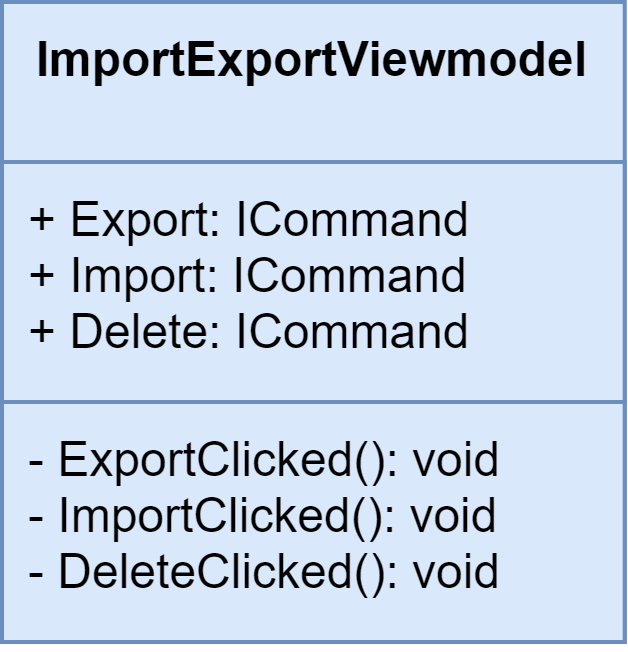
\includegraphics[width=\textwidth]{bilder/ViewmodelKlassen/ImportExportViewmodel}
\end{minipage}
\paragraph{Klassenbeschreibung:}
Das ImportExportViewmodel verarbeitet das Klicken des Nutzers auf die Buttons  der ImportExportPage.
Die Kommunikation wird dabei mit Commands geregelt.
\paragraph{Attribute:}
\begin{itemize}
	\item[+] \textbf{Export: ICommand}
	\item[+] \textbf{Import: ICommand}
	\item[+] \textbf{Delete: ICommand}
\end{itemize}
Die Commands werden je an den entsprechenden Button im View gekoppelt und lösen die entsprechende Methode in dieser Klasse aus.
\paragraph{Methoden:}
\begin{itemize}
    \item[$-$] \textbf{exportClicked(): void}\\ öffnet einen folderPicker-Dialog und ruft danach in IDataBaseConnection exportTrainingData mit dem vom Nutzer im Dialog ausgewählten Pfad aus.%%??name genau von dem filePicker??
    \item[$-$] \textbf{importClicked(): void}\\ öffnet einen filePicker-Dialog und ruft danach in IDataBaseConnection importTrainingData mit dem vom Nutzer ausgewählten file auf.
    \item[$-$] \textbf{deleteClicked(): void}\\zeigt einen Warning-Dialog an, ob man wirklich alle Vorgangsdaten löschen will. Daraufhin wird bei Bestätigung in IDatabaseConnection deleteTrainingData aufgerufen.
\end{itemize} 

\begin{minipage}[b]{0.7\textwidth}

	\subsection{Class SettingsViewModel}
\end{minipage}
\begin{minipage}[c]{0.3\textwidth}
	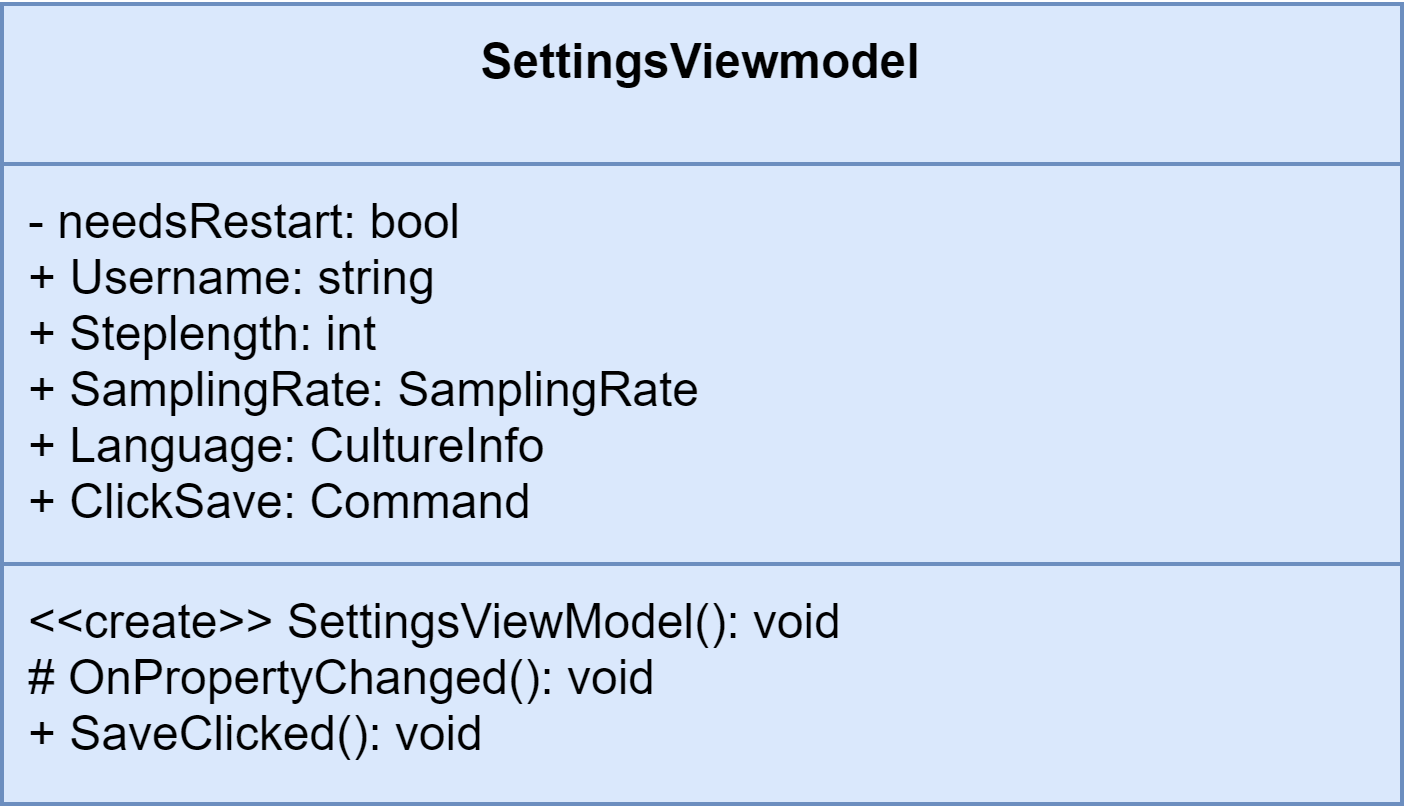
\includegraphics[width=\textwidth]{bilder/ViewmodelKlassen/SettingsViewModel.png}
\end{minipage}
\paragraph{Klassenbeschreibung:}
Die Klasse SettingsViewModel enthält die Logik der SettingsPage. Sie erbt von INotifyPropertyChanged und verwendet für das Speichern der Einstellungen einen Command. Außerdem holt sie sich vom SettingsService alle aktuellen Einstellungen.
\paragraph{Attribute:}
\begin{itemize}
	\item[$-$] \textbf{needsRestart: bool}\\ diese Property verfügt nur über einen privaten getter. Sie ist genau dann wahr, wenn der Nutzer die Sprache geändert hat, also der Zustand des Sliders in der View und der Zustand als in dieser Klasse als Attribut gespeicherten Sprache unterschiedlich sind.
	\item[+] \textbf{Username: String}\\Der Username verfügt über ein Binding zur View.
	\item[+] \textbf{StepLength: int}\\Die StepLength verfügt über ein Binding zur View. 
	\item[+] \textbf{SamplingRate: SamplingRate}\\Die SamplingRate wird nicht direkt im View gebindet.
	\item[+] \textbf{Language: CultureInfo}\\Die Language wird nicht direkt im View gebindet. 
	\item[+] \textbf{ClickSave: Command}\\Bei Ausführen dieses Commands wird die Methode SaveClicked ausgeführt. 
\end{itemize}
\paragraph{Methoden:}
\begin{itemize}
    \item[+] \textbf{<<create>> SettingsViewModel(): void}\\ Im Konstruktor holt sich die Klasse vom ISettingsService den User, die Sprache und die Samplingrate und speichert die Entsprechenden Werte in den eigenen Properties. Die Werte von Attributen, die über kein Binding verfügen, müssen hier manuell ins View übertragen werden.
    \item[#] \textbf{OnPropertyChanged(): void} Die Methode wird von der Schnittstelle INotifyPropertyChanged geerbt. Diese wird benutzt um die View zu aktualisieren und ihr um Bescheid zu geben, wenn sich eine Eigenschaft aus dem ViewModel verändert. 
    \item[$-$] \textbf{SaveClicked(): void}\\ wenn diese Methode aufgerufen wird, werden die aktuellen Properties wieder im ISettingsService gespeichert, nachdem alle Werte von Attributen, die über kein Binding verfügen, vom View geholt und aktualisiert werden. Außerdem wird die Schrittlänge ans Erweiterungsmodul und die Samplingrate an die Bibliothek weitergegeben. Bei Auftretenden Exceptions (kein Gerät verbunden) wird eine Fehlermeldung als Popup angezeigt. Liefert needsRestart wahr, wird außerdem ein Hinweis angezeigt, dass die App neu gestartet werden muss, um alle Änderungen zu übernehmen. 
\end{itemize} 

\subsection{Class ScanningPopUpViewModel}
	\paragraph{Klassenbeschreibung:}
	Die Klasse ScanningPopUpViewModel ist das ViewModel zu dem View PopUpScanningPage und verwaltet die Logik dieser Komponente mithilfe von verknüpften Commands. Dabei implementiert die Klasse die Schnittstelle INotifyPropertyChanged, um die View zu aktuallisieren.
	Sie benutzt die Erweiterung \Gls{Rg.Plugins.Popup} für das Anzeigen und das Versteckend des Pop-ups.
	
	\paragraph{Attribute:}
	\begin{itemize}
		\item[+] \textbf{static IsConnected: bool}\\Statisches Attribut, ob das Gerät mit den \gls{Earables} verbunden ist.
		\item[+] \textbf{ScanDevicesCommand: ICommand}\\Command, welches die Implementierung des Scannen abkapselt. Dieses Command wird ausgeführt, wenn der ScanDevice Button im View betätigt wird. Es wird die private Methode ScanDevices() aufgerufen.
		\item[+] \textbf{ConnectDeviceCommand: ICommand}\\Command, welches die Implementierung des Verbinden mit einem ausgewählten BLE Gerät aus dem ListView des Pop-ups. Es wird die private Methode ConnectDevice() aufgerufen.
		\item[+] \textbf{CancelCommand: ICommand}\\Command, welches die Implementierung des Abbrechen abkapselt. Dieses Command wird ausgeführt, wenn der Cancel Button im View betätigt wird. Es wird die public und statische Methode HidePopUp() aufgerufen. 
		\item[+] \textbf{Devices: ObservableCollection<Device>}\\Die Liste Devices dient zur Aktuallisierung des Views PopUpScanningPage. Die ListView im View setzt Devices als Ressource. Da Devices eine ObservableCollection ist, wird die Listview bei einer Änderung der Deviceliste aktualisiert.
	\end{itemize}

	\paragraph{Methoden:}
	\begin{itemize}
		\item[+] \textbf{<<create>> ScanningPopUpViewModel()}\\Der Konstruktor für die Klasse ScanningPopUpViewModel. In dieser Methode, werden die Commands initialisiert. Zudem wird sich bei dem EventHandler DeviceConnectionStateChanged in der Klasse EarablesConnection im Model mit der Methode OnDeviceConnectionStateChanged(...) registriert.
		\item[\#] \textbf{OnPropertyChanged(): void}\\Die Methode wird von der Schnittstelle INotifyPropertyChanged geerbt. Diese wird benutzt um die View zu aktualisieren und ihr um Bescheid zu geben, wenn sich eine Eigenschaft aus dem ViewModel verändert.
		\item[+] \textbf{OnDeviceConnectionStateChanged(sender: object, args: DeviceEventArgs): void}\\Mit dieser Methode registrierst das ViewModel bei dem EventHandler DeviceConnectionStateChanged. In dieser wird das statische Attribut IsConnected angepasst. Falls sich das Device disconnected hat, wird die Methode ShowPopUp() aufgerufen.
		\item[$-$] \textbf{ScanDevices(): void}\\Private Methode, welche im Command ConnectDeviceCommand benutzt wird. In dieser wird die EarableConnection nach erreichbaren Geräten gefragt. Dafür wird die Methode StartScanning() aufgerufen. Die zurückgelieferte Liste an Devices wird in dem Pop-up angezeigt. Dafür wird die ListView aktualisiert. Zudem wird das erste Device in der ListView ausgewählt.
		\item[$-$] \textbf{ConnectDevice(): void}\\Private Methode, welche im Command ConnectDeviceCommand aufgerufen wird. Dabei benutzt sie die Methode ConnectToDevice(device: IDevice) der Klasse EarableConnection im Model. Es wird das Device übergeben, welches in der ListView ausgewählt wurde.
		\item[+] \textbf{static ShowPopUp(): void}\\Statische Methode, welche die View PopUpScanningPage anzeigt. Diese benutzt die Erweiterung \Gls{Rg.Plugins.Popup}. Das Anzeigen geschieht mit der Methode Popupnavigation.Instance.PushAsync(new PopUpScanningPage()). Dabei wird ein neue Instanz der PopUpScanningPage erstellt. Die Methode ist statisch, da die anderen ViewModels bei einem Vorgangstart anzeigen können muss, falls noch keine Verbindung zu den \gls{Earables} besteht.
		\item[+] \textbf{static HidePopUp(): void}\\Statische Methode, welche dieView PopUpScanningPage verstecken lässt. Diese Methode benutzt die Erweiterung \Gls{Rg.Plugins.Popup}. Das Verstecken der View geschieht mit der Methode Popupnavigation.Instance.popAsync(). 
	\end{itemize}
\begin{minipage}[b]{0.7\textwidth}

	\subsection{Class HomeMenuItem}
\end{minipage}
\begin{minipage}[c]{0.3\textwidth}
	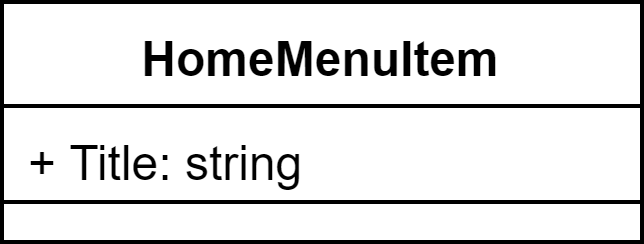
\includegraphics[width=\textwidth]{bilder/ViewmodelKlassen/HomeMenuItem.png}
\end{minipage}
	\paragraph{Klassenbeschreibung:}
	Diese Klasse spezifiziert einen Eintrag des Menüs (siehe MenuPage). 
	\paragraph{Attribute:}
	\begin{itemize}
		\item [+] \textbf{Id: MenuItemType}\\ Der Typ des Menüeintrags (in UML als Assozation dargestellt).
		\item [+] \textbf{Title: string}\\ Der angezeigte Text des Menüeintrags.
	\end{itemize}
\begin{minipage}[b]{0.7\textwidth}

	\subsection{Enumeration MenuItemType}
\end{minipage}
\begin{minipage}[c]{0.3\textwidth}
	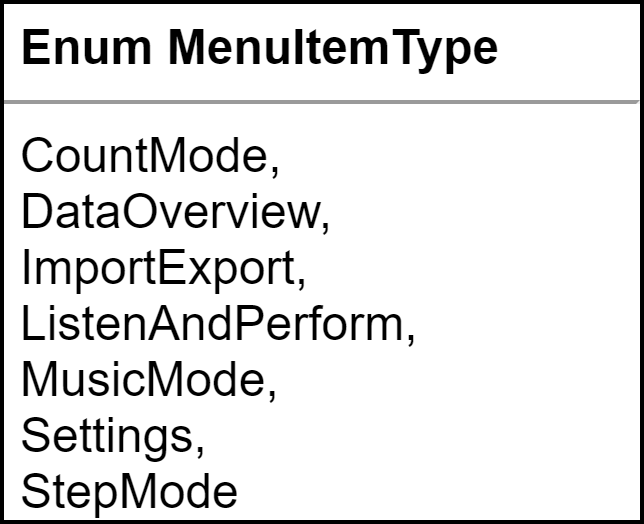
\includegraphics[width=\textwidth]{bilder/ViewmodelKlassen/MenuItemType.png}
	\vspace{0.3cm}
\end{minipage}

	Dieses Enum spezifiziert alle möglichen Typen von Menüeinträgen der MenuPage. Entsprechend gibt es für jede vom Menü aus direkt navigierbare Page einen Wert dieses Enums.\\
	\paragraph{Werte:}
	\begin{itemize}
        \item CountMode,
        \item DataOverview,
        \item ImportExport,
        \item ListenAndPerform,
        \item MusicMode,
        \item Settings,
        \item StepMode
	\end{itemize}

\subsection{Class ExceptionHandlingViewModel}
	\paragraph{Klassenbeschreibung:}
	Die Klasse ExceptionHandlingViewModel ist die zentrale Fehlerverarbeitung. Wenn eine Exception in anderen Komponenten des ViewModels oder des Models wird die Exception gefangen und an die Klasse ExceptionHandlingViewModel weitergeleitet. Diese erstellt nun eine Benachrichtigung in Form eines DisplayAlert, sodass der Nutzer von dieser Exception erfährt. 
	
	\paragraph{Methoden:}
	\begin{itemize}
		\item[+] \textbf{static HandleException(error: Exception): void}\\Die statische Methode HandleException nimmt als Parameter eine Instanz der Klasse Exception. In dieser Methode wird ein DisplayAlert erstellt mit dem Titel der Exception und dessen Inhalt. Dies wird mit einer Referenz auf die MainPage getan.
	\end{itemize}
\section{Klassenbeschreibung View}


\subsection{Class StepModePage}
\paragraph{Klassenbeschreibung:}
Diese Klasse stellt die Ansicht des StepModes dar, solange kein Laufvorgang gestartet ist.
\paragraph{Attribute:}
	\begin{itemize}
	\item[+] \textbf{StepMode: Label} \\ Anzeige des Modusnamen Stepmode.
	\item[+] \textbf{LastTrainingsDate: Label} \\ Anzeige für den letzten Trainingstag, an das Attribut LastDataTime aus dem Viewmodel gebunden.
	\item[+] \textbf{StepsDoneLastTime: Label} \\ Anzeige für die am letzten Trainingstag gelaufenen Schritte, an das Attribut StepsDoneLastTIme aus dem Viewmodel gebunden.
	\item[+] \textbf{DistanceWalkedLastTime: Label} \\ Anzeige für die am letzten Trainingstag gelaufene Distanz, an das Attribut DistanceWalkedLastTime aus dem Viewmodel gebunden. 
	\item[+] \textbf{Start: Button} \\ Button um den Laufvorgang zu starten. Feuert den StartActivityCommand aus dem Viewmodel.
	\end{itemize}

\subsection{Class StepModeActivePage}
\paragraph{Klassenbeschreibung:}
Diese Klasse stellt die Ansicht des Stepmodes während eines laufenden Laufvorgangs an.
\paragraph{Attribute:}
	\begin{itemize}
	\item[+] \textbf{StepMode: Label} \\ Anzeige des Modusnamen Stepmode.
	\item[+] \textbf{IsRunning: Label} \\ Zeigt an ob der Nutzer aktuell läuft oder steht, an das Attribut IsRunning aus dem Viewmodel gebunden.
	\item[+] \textbf{StepCounter: Label} \\ Anzeige für Anzahl bisher gelaufener Schritte, an das Attribut StepCounter aus dem Viewmodel gebunden.
	\item[+] \textbf{DistanceWalked: Label} \\ Anzeige der bisher gelaufenen Distanz, an das Attribut DistanceWalked aus dem Viewmodel gebunden.
	\item[+] \textbf{StepFrequency: Label} \\ Anzeige der akutellen Schrittfrequenz, an das Attribut StepFrequency aus dem Viewmodel gebunden.
	\item[+] \textbf{Stop: Button} \\ Button um den Laufvorgang zu stoppen. Feuert den StopActivityCommand aus dem Viewmodel.
	\end{itemize}
	
\subsection{Class CountModePage}
\paragraph{Klassenbeschreibung:}
Diese Klasse stellt die Ansicht des Countmodes dar, solange kein Zählvorgang gestartet ist.
\paragraph{Attribute:}
	\begin{itemize}
	\item[+] \textbf{CountMode: Label} \\ Anzeige des Modusnamen CountMode.
	\item[+] \textbf{Activities: ListView} \\ Anzeige der verfügbaren Activities die auswählbar sind mithilfe einer ListView, an die ObservableCollection PossibleActivities aus dem Viewmodel gebunden.
	\item[+] \textbf{Start: Button} \\ Button um den Zählvorgang zu starten. Feuert den StartActivityCommand aus dem Viewmodel.
	\end{itemize}

\subsection{Class CountModeActivePage}
\paragraph{Klassenbeschreibung:}
Diese Klasse stellt die Ansicht des Countmodes während eines laufenden Zählvorgangs an.
\paragraph{Attribute:}
	\begin{itemize}
	\item[+] \textbf{CountMode: Label} \\ Anzeige des Modusnamen CountMode.
	\item[+] \textbf{Timer: Label} \\ Anzeige für die seit dem Zählstart vergangene Zeit. Beinhaltet drei Spans für die Anzeige von Minuten, Sekunden und Millisekunden. Das Spans sind an die Attribute Minuten, Sekunden bzw. Millisekunden gebunden.
	\item[+] \textbf{Counter: Label} \\ Anzeige für die Anzahl bisher ausgeführter Wiederholungen einer Activity. An das Attribut Counter aus dem Viewmodel gebunden.
	\item[+] \textbf{SelectedActivity: Label} \\Anzeige für die ausgewählte Übung. An das Attribut SelectedActivity aus dem Viewmodel gebunden.
	\item[+] \textbf{Stop: Button} \\ Button um den Zählvorgang zu stoppen. Feuert den StopActivityCommand aus dem Viewmodel.
	\end{itemize}

\subsection{Class ListenAndPerformPage}
\paragraph{Klassenbeschreibung:}
Diese Klasse stellt die Ansicht von ListAndPerform dar, solange kein Trainingsvorgang gestartet ist.
\paragraph{Attribute:}
	\begin{itemize}
	\item[+] \textbf{ListenAndPerform: Label} \\ Anzeige des Modusnamen ListenAndPerform.
	\item[+] \textbf{WorkoutPlan: Label} \\ Anzeige vom Schriftzug Workout plan.
	\item[+] \textbf{Activities: ListView} \\	Anzeige für den bisher zusammengestellten Trainingsplan mithilfe einer ListView, an das Attribut ActivityList gebunden. 
	\item[+] \textbf{AddActivity: Button} \\ Button um eine Activity dem Trainingsplan hinzuzufügen. Feuert den AddActivityCommand aus dem Viewmodel.
	\item[+] \textbf{RemoveActivity: Button} \\ Button um eine Activity aus dem Trainingsplan zu löschen. Feuert den RemoveActivityCommand aus dem Viewmodel.
	\item[+] \textbf{EditActivity: Button} \\ Button um eine bereits hinzugefügte Activity oder ihre Anzahl zu ändern. Feuert den EditActivityCommand aus dem Viewmodel.
	\item[+] \textbf{Start: Button} \\ Button um den Trainingsvorgang zu starten. Feuert den StartActivityCommand aus dem Viewmodel.
	\end{itemize}

\subsection{Class ListenAndPerformActivePage}
\paragraph{Klassenbeschreibung:}
Die Klasse stellt die Ansicht von ListenAndPerform während eines laufenden Trainingsvorgangs an.
\paragraph{Attribute:}
	\begin{itemize}
	\item[+] \textbf{ListenAndPerform: Label} \\ Anzeige des Modusnamen ListenAndPerform.
	\item[+] \textbf{Activity: Label} \\ Anzeige für die aktuell auszuführenden Activity.
	\item[+] \textbf{Timer: Label} \\ Anzeige für die seit dem Zählstart vergangene Zeit. Beinhaltet drei Spans für die Anzeige von Minuten, Sekunden und Millisekunden. Das Spans sind an die Attribute Minuten, Sekunden bzw. Millisekunden gebunden.
	\item[+] \textbf{Counter: Label} \\ Anzeige für die Anzahl bisher ausgeführter Wiederholungen einer Activity. An die Attribute PushUpCounter und SitUpCounter aus dem Viewmodel gebunden.
	\item[+] \textbf{Progress: ProgressBar} \\ Progressbar zum Anzeigen des Fortschritts innerhalb einer Activity.
	\item[+] \textbf{Stop: Button} \\ Button um den Trainingsvorgang zu stoppen. Feuert den StopActivityCommand aus dem Viewmodel.
	\end{itemize}
	
\subsection{Class MusicModePage}
\paragraph{Klassenbeschreibung:}
Die Klasse stellt die komplette Ansicht des Musicmodes dar. Beim Starten des Musikvorgang wird zu keiner Page gewechselt.
\paragraph{Attribute:}
	\begin{itemize}
	\item[+] \textbf{MusicMode: Label} \\ Anzeige des Modusnamen MusicMode.
	\item[+] \textbf{TwoWayButton: Label} \\ Button um den Musikvorgang zu Starten/Stoppen. Feuert beim Starten/Stoppen den StartActivityCommand und den StopActivityCommand respektive.
	\end{itemize}

	\subsection{Class DataOverviewPage}
		\paragraph{Klassenbeschreibung:}
		Diese Seite soll dem Nutzer die Ansicht seiner letzten Trainingsergebnisse ermöglichen.
		Die Daten werden dabei vom DataOverviewViewModel per Data-Binding bereit gestellt.
		\paragraph{Attribute:}
		\begin{itemize}
			\item[+] \textbf{ContentListView: ListView}
			\item[+] \textbf{BindingContext: DataOverviewViewModel} 
		\end{itemize}

	
\begin{minipage}[b]{0.7\textwidth}

	\subsection{Class ImportExportPage}

\end{minipage}
\begin{minipage}[c]{0.3\textwidth}
	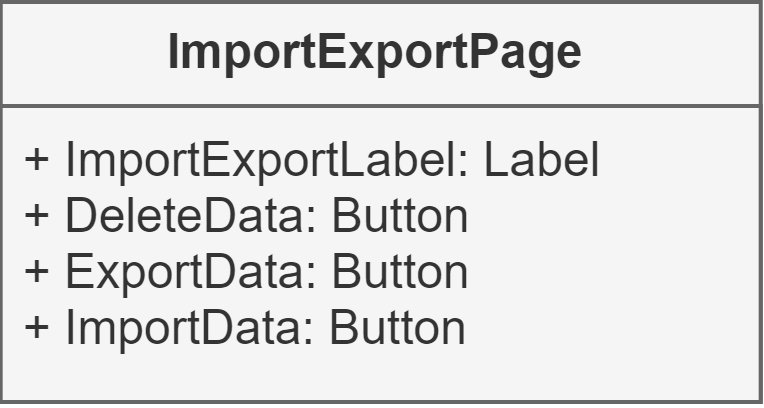
\includegraphics[width=\textwidth]{bilder/ViewKlassen/ImportExportPage.png}
\end{minipage}
		\paragraph{Klassenbeschreibung:}
		Die Klasse ImportExportPage beinhaltet eine Seite mit drei Buttons (siehe Abbildung 11 (Seite 13) im Pflichtenheft).
		Das Klicken auf diese Buttons benachrichtigt das ImportExportViewmodel (via Command).
		\paragraph{Attribute}
		\begin{itemize}
			\item[+] \textbf{ImportExportLabel: Label} \\ Anzeige des Pagenamens (Im-/ Export CSV Datei).
			\item [+]\textbf{DeleteData: Button}
			\item [+]\textbf{ExportData: Button}
			\item [+]\textbf{ImportData: Button} %%die anderen haben es auch public gemacht - einheitlich. ist das sinnvoll oder kann das private? -valle
		\end{itemize}

	\begin{minipage}[b]{0.7\textwidth}

		\subsection{Class SettingsPage}
	\end{minipage}
	\begin{minipage}[c]{0.3\textwidth}
		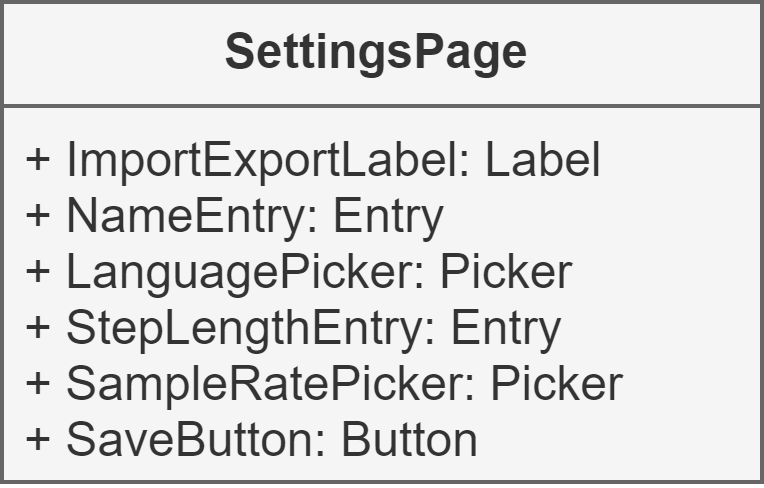
\includegraphics[width=\textwidth]{bilder/ViewKlassen/SettingsPage.png}
	\end{minipage}
		\paragraph{Klassenbeschreibung:}
		Die Einstellungsseite ermöglicht das Verändern und Einsehen von Username, Sprache, Schrittlänge und IMU-Samplingrate (Siehe Abb. 12 im Pflichtenheft). Die Daten werden per Data-Binding mit der Klasse SettingsViewModel synchronisiert.
		\paragraph{Attribute}
		\begin{itemize}
			\item[+] \textbf{ImportExportLabel: Label} \\ Anzeige des Pagenamens (Settings).
			\item [+]\textbf{NameEntry: Entry}
			\item [+]\textbf{LanguagePicker: Picker} Hier kann der Nutzer zwischen Deutsch und Englisch wählen.
			\item [+]\textbf{StepLengthEntry: Entry} 
			\item [+]\textbf{SampleRatePicker: Picker} Hier kann der Nutzer zwischen wenigen angebotenen Samplingraten wählen. Diese entsprechen denen vom Settings Service zur Verfügung gestellten Werte.
			\item [+]\textbf{SaveButton: Button}
		\end{itemize}

	\subsection{Class PopUpScanningPage}
		\paragraph{Klassenbeschreibung:}
		Die Klasse erbt von der Klasse PopupPage aus der Erweiterung \Gls{Rg.Plugins.Popup}, welche die Grundstruktur eines Pop-up Fenster implementiert.\\
		Die Klasse PopUpScanningPage beinhaltet das Pop-up, welches erscheint, wenn keine Verbindung zu den \gls{Earables} besteht. Dies wird überprüft, wenn die App geöffnet wird oder ein Vorgang gestartet werden soll. Dabei interagiert das Pop-Up mit dem Model (der Bibliothek), welches die Verbindungssuche und die Verbindung implementiert. Bei einer erfolgreichen Verbindung, verschwindet das Pop-Up automatisch; bei einer fehlerhaften Verbindung wird eine Fehlermeldung angezeigt. Der Nutzer kann das Pop-Up mit dem 'Cancel-Button' wegklicken. 
		\paragraph{Attribute}
		\begin{itemize}
		\item[+] \textbf{Alert: Label}\\Ein Label, welches die Benachrichtigung anzeigt, dass die Verbindung zu den \gls{Earables} nicht besteht. Bei einem fehlgeschlagenen Verbindungsversuch färbt es sich kurzartig rot.
		\item[+] \textbf{ScanDevices: Button}\\Schickt das Command ab, welches die Bibliothek nach \gls{Earables} suchen lässt.
		\item[+] \textbf{DevicesAvailable: ListView}\\Liste der \Gls{Earables} mit denen man sich per \gls{BLE} verbinden kann. Es ermöglicht einem einen Eintrag auszuwählen. Die Liste wird von dem Viewmodel ScanningPopUpViewModel aus aktualisiert.
		\item[+] \textbf{ConnectButton: Button}\\Schickt das Command ab, welches der Bibliothek mitteilt mit den \Gls{Earables} zu verbinden, welche im ListView ausgewählt wurde.
		\item[+] \textbf{Cancel: Button}\\Schickt das Command ab, welches das Pop-up verschwinden lässt. Es wurde keine Verbindung hergestellt.
		\item[+] \textbf{BindingContext: ScanningPopUpViewModel}\\Der BindingContext ist vom Typ ScanningPopUpViewModel, welches die einzelnen UI-Komponenten des Pop-ups aktualisiert. Hier sind ebenfalls die Commands implementiert.
		\end{itemize}
		
		\paragraph{Methoden}
		\begin{itemize}
		\item[+] \textbf{<<create>> PopUpScanningPage}\\Konstruktor der Klasse PopUpScanningPage. In diesem wird eine Instanz des ViewModels und BindingContext der Klasse ScanningpopUpViewModel erstellt.
		\end{itemize}

		\begin{minipage}[b]{0.7\textwidth}

			\subsection{Class MainPage}
		\end{minipage}
		\begin{minipage}[c]{0.3\textwidth}
			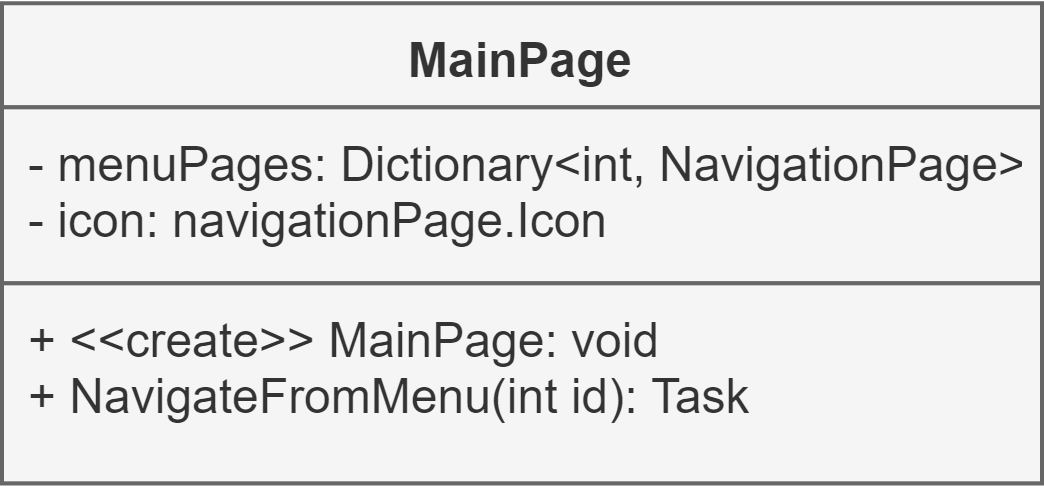
\includegraphics[width=\textwidth]{bilder/ViewKlassen/MainPage.png}
		\end{minipage}
		\paragraph{Klassenbeschreibung:}
		Die MainPage erbt von MasterDetailPage und stellt die grundlegende angezeigte Struktur zur Verfügung. Das ist im Wesentlichen der Menü-Button (vlg. Preset "MasterDetailPage" in Visual Studio 2019).\\
		Bei Klicken auf das Menü-Icon bzw. swipen vom Rand aus öffnet sich automatisch (vererbt von MasterDetailPage) die MenuPage.
		\paragraph{Attribute}
		\begin{itemize}
			\item [-] \textbf{MenuPages: Dictionary<int, NavigationPage>}\\ Dieses Dictionary wird verwendet, um mit dem Klicken auf den Namen einer bestimmten Page die Page selbst zu assoziieren (bzw. die ihr entsprechende NavigationPage).
			\item [-] \textbf{icon: navigationPage.Icon} Das Menü-Item, das sich für den Nutzer links oben im Eck befindet.
		\end{itemize}
		\paragraph{Methoden}
		\begin{itemize}
			\item [+] \textbf{<<create>> MainPage: void}\\ Hier wird die Seite initialisiert. Dazu wird der Laufmodus als aktuelle DetailPage festgelegt.
			\item [+] \textbf{NavigateFromMenu(int id): Task}\\ Diese Methode setzt die zur angegebenen ID entsprechende Page als neue DetailPage fest.
		\end{itemize}
	\begin{minipage}[b]{0.7\textwidth}

		\subsection{Class MenuPage}
	\end{minipage}
	\begin{minipage}[c]{0.3\textwidth}
		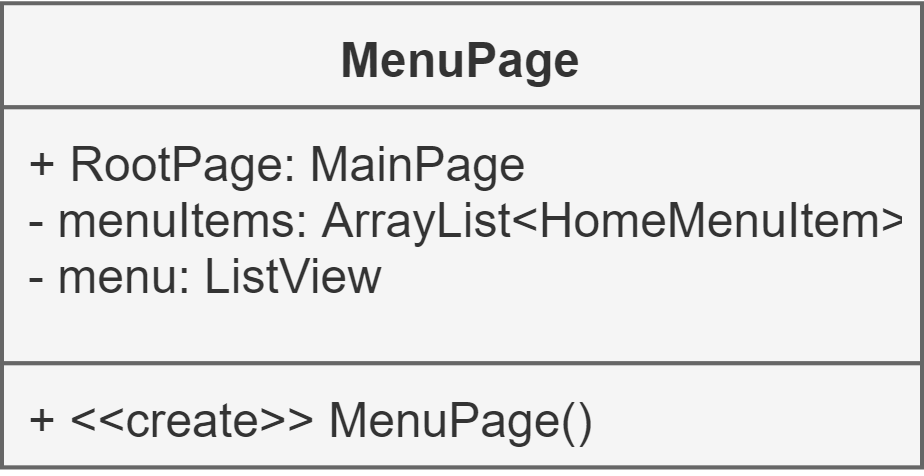
\includegraphics[width=\textwidth]{bilder/ViewKlassen/MenuPage.png}
	\end{minipage}
		\paragraph{Klassenbeschreibung:}
		Die MenuPage ist das Menü, aus dem der Nutzer nach Klicken des Menü-Buttons eine Seite auswählen kann.
		\paragraph{Attribute}
		\begin{itemize}
			\item [+] \textbf{RootPage: MainPage} Diese Property verfügt nur über einen Getter, der die aktuelle MainPage zurückgibt.
			\item [-] \textbf{menuItems: List<HomeMenuItem>} Diese Liste enthält alle von der MenuPage aus direkt ansteuerbaren Seiten.
			\item [-] \textbf{menu: ListView} Das menu ist das menuItems entsprechende angezeigte Element auf der Seite.		
		\end{itemize}
		\paragraph{Methoden}
		\begin{itemize}
			\item [+] \textbf{<<create>> MenuPage()} Im Konstruktor wird menuItems mit allen gewünschten Seiten initialisiert und den menuItems wird ein Event, das bei Auswählen eines Items gefeuert wird, hinzugefügt. Dieses veranlasst die Navigation zu dieser Seite mittels der MainPage.
		\end{itemize}
	
\newpage
\section{Interaktionsdiagramme}
\subsection{Aktivitätsdiagramm Lebenszyklus der App}
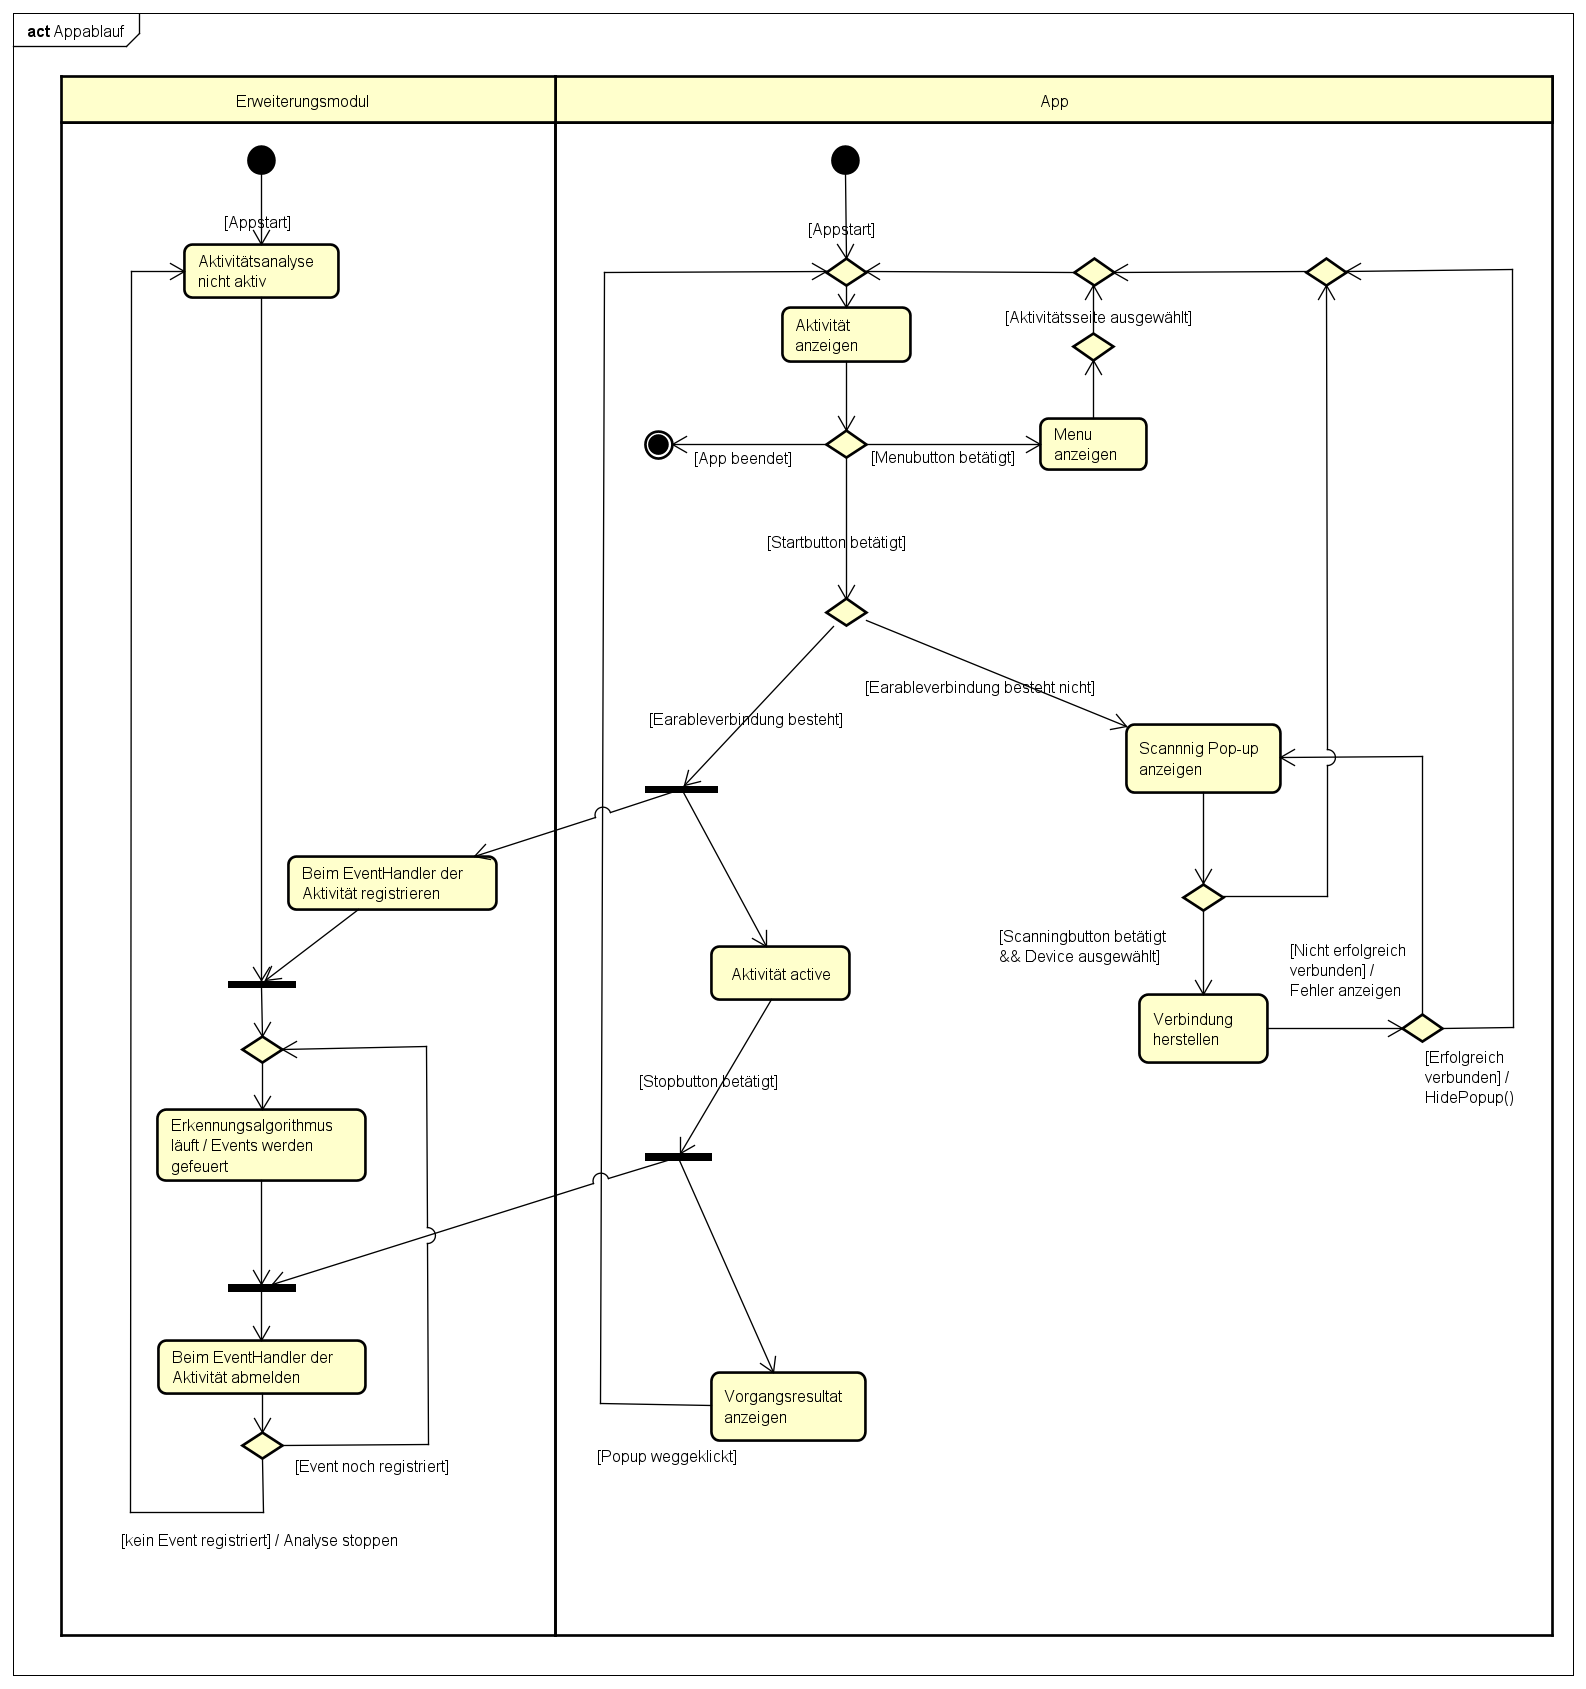
\includegraphics[width=1.1\textwidth]{./Diagramme/Appablauf.png}
\subsection{Sequenzdiagramme}


%später:
%brauchen wir den unterpunkt "abläufe in der app" alle sqd die wir haben beziehen sich doch auch auf die App
\subsubsection{Abläufe in der App}

\paragraph{Start der App}

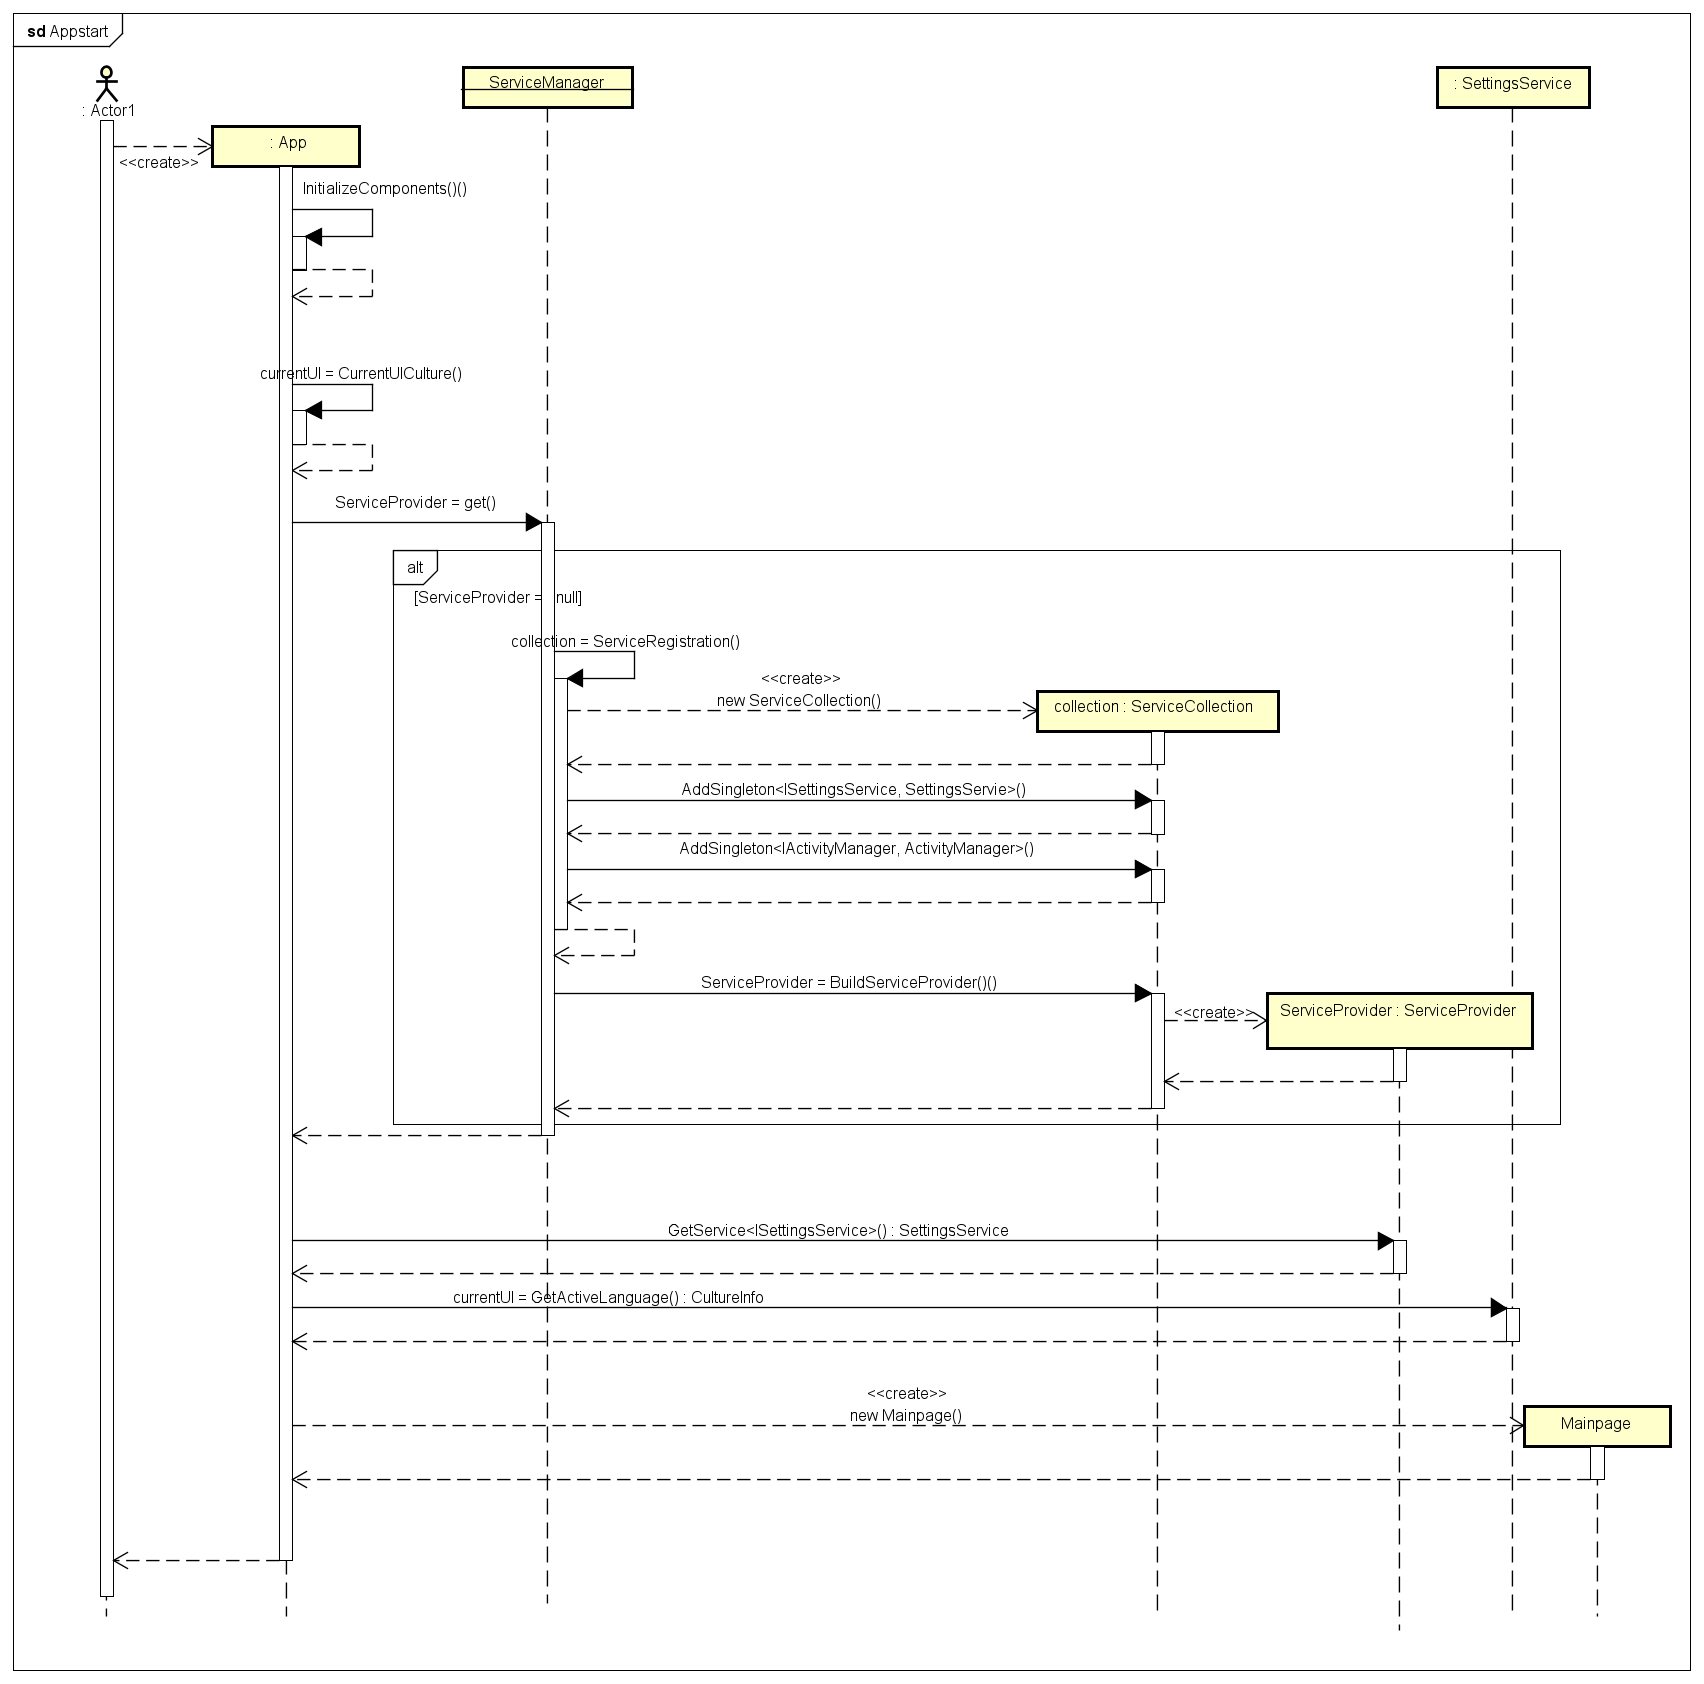
\includegraphics[width=1.1\textwidth]{./Diagramme/AppstartSeqDia.png}


\paragraph{Bluetoothverbindung mit den Earables herstellen:}
Das folgende Sequenzdiagramm verdeutlicht wie eine Bluetoothverbindung hergestellt werden kann. Es wir davon ausgegangen, dass die App bereits gestartet wurde und noch keine Bluetoothverbindung zu den Earables besteht. Außerdem zeigt die App geraden die Seite des Laufmodus an und das PopUpViemwmodel kennt den Service der EarablesConnection bereits.\\

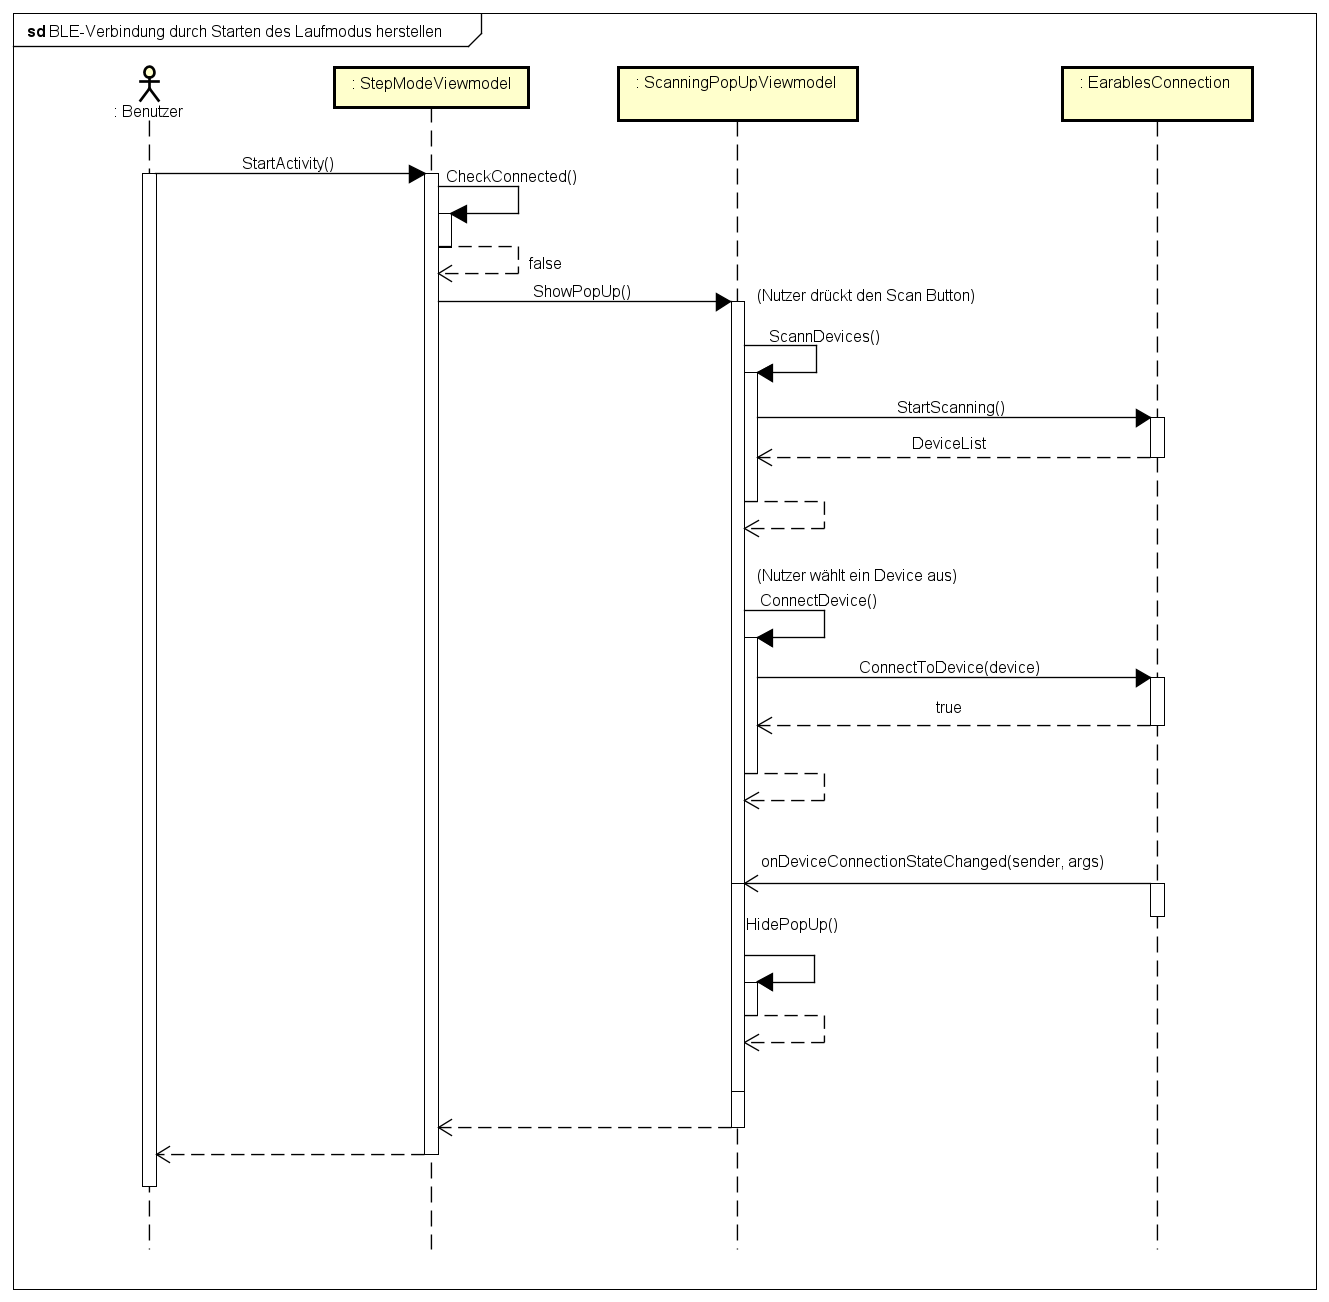
\includegraphics[width=1.1\textwidth]{./Diagramme/Verbindungsaufbausequenzdiagramm.png}

\paragraph{Navigationsmenu Page auswählen}

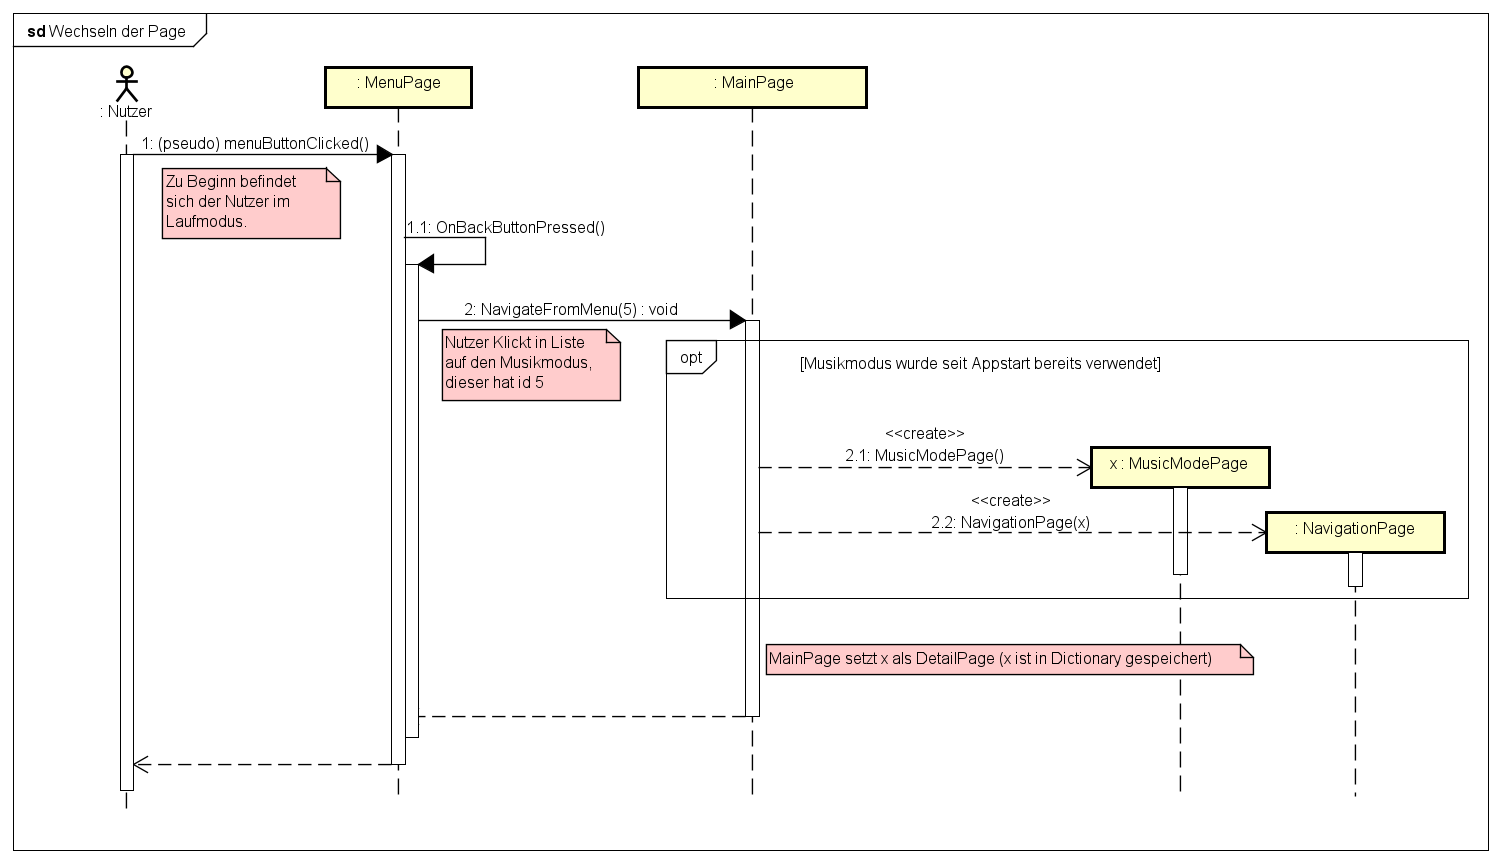
\includegraphics[width=1.1\textwidth]{./Diagramme/NavigationsMenuSeqDia.png}


\paragraph{Zählvorgang}
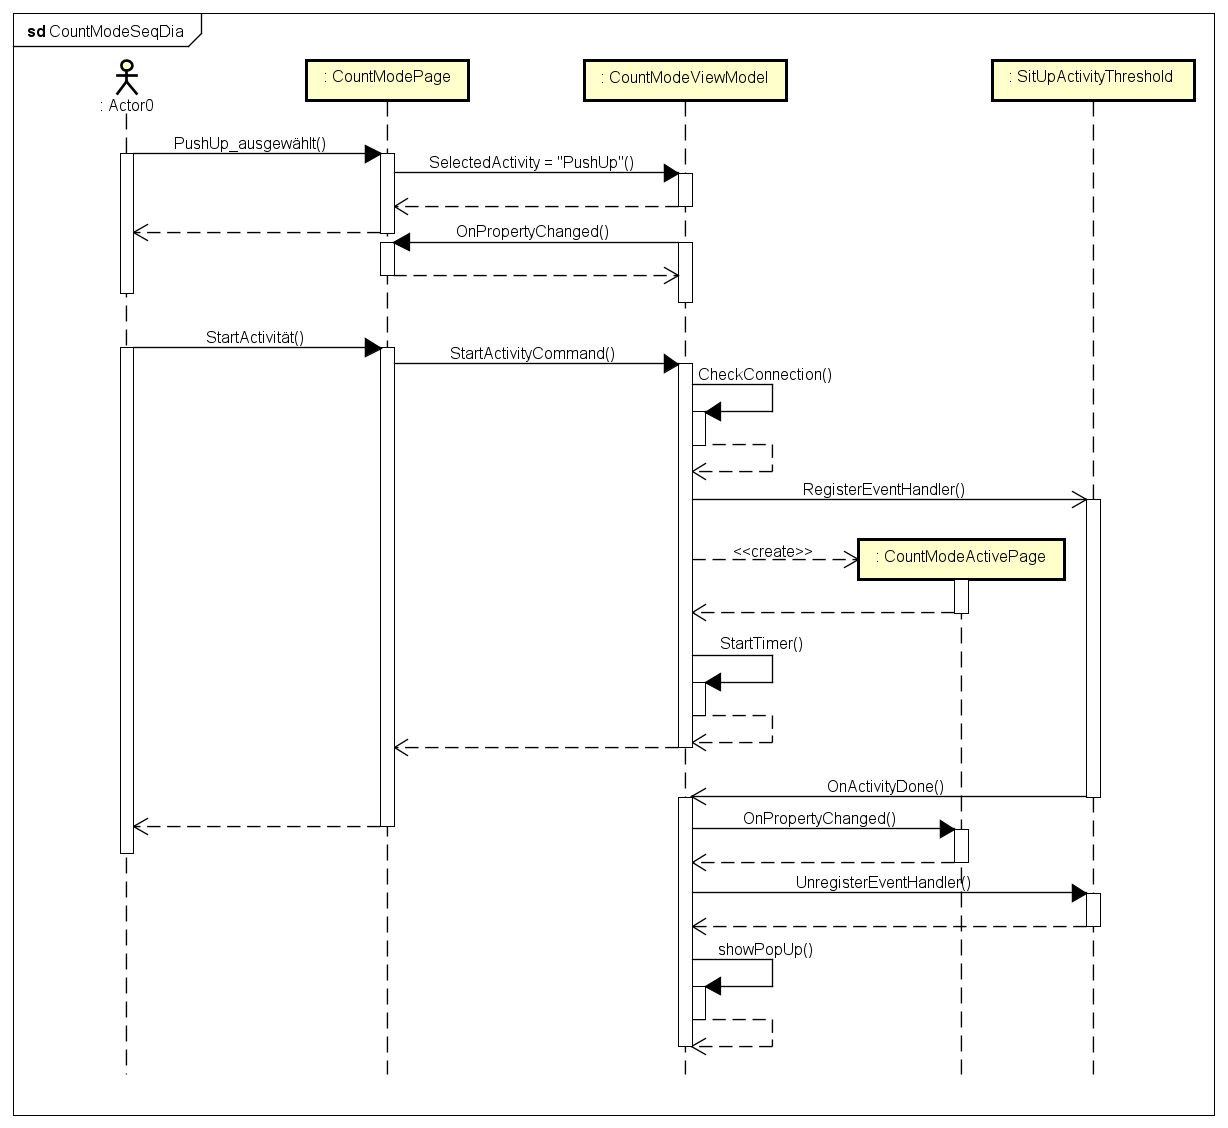
\includegraphics[width=1.1\textwidth]{./Diagramme/CountModeSeqDia.png}


\paragraph{Export Trainingsdaten:}
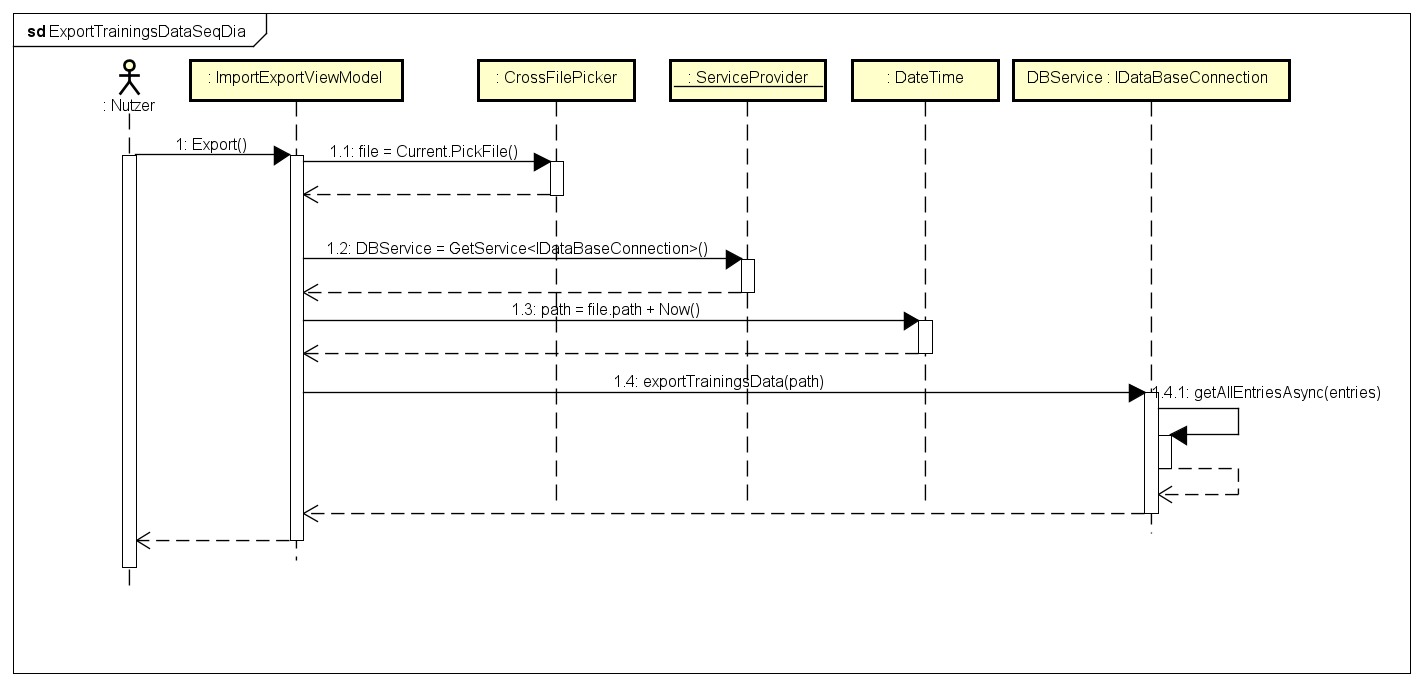
\includegraphics[width=1.1\textwidth]{./Diagramme/TrainingsDatenExport_Sequenz.png}

\paragraph{Änderung der Samplerate:}
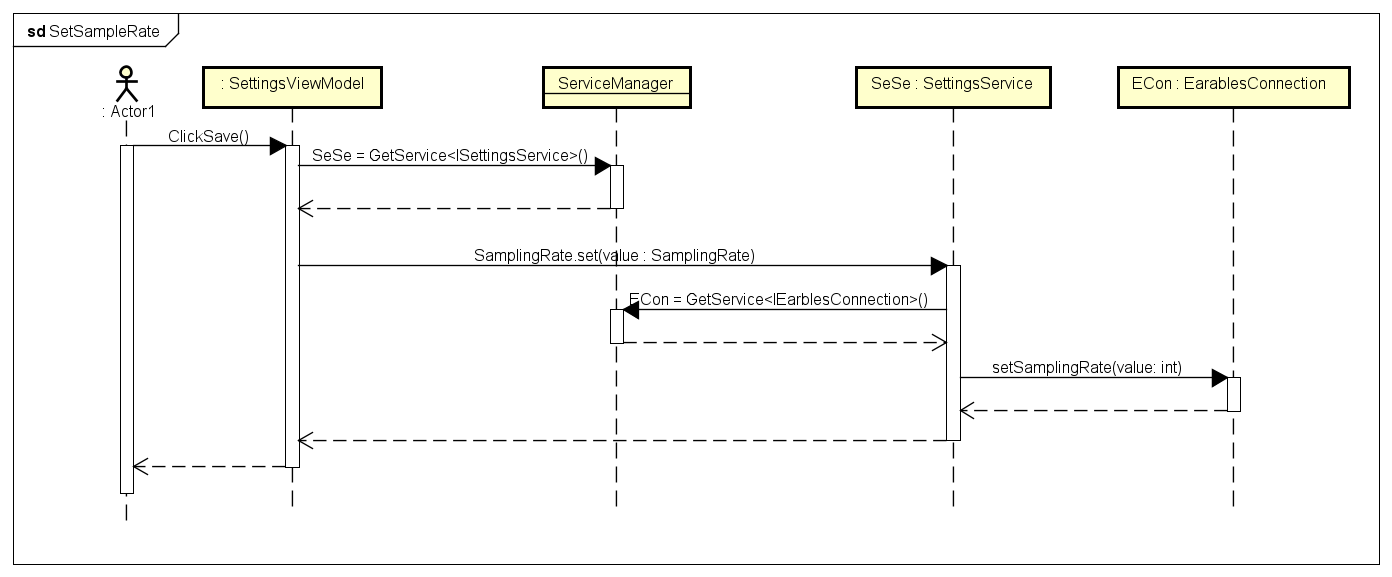
\includegraphics[width=1.1\textwidth]{./Diagramme/SetSampleRateSeqDia.png}

\section{Entwurfdaten}
\subsection{Ressourcenverzeichnis}
\subsection{lokale Datenbank}
\subsection{App Properties}

\section{Klassenindex}
%macht valle ganz am Ende oder wir lassen es weg
\section{Anhang}

%%%%%%%%%%%%%%%%%%%%%%%%%%%%%%%%%%%%%%% END CONTENT %%%%%%%%%%%%%%%%%%%%%%%%%%%%%%%%%%%%%%%%%%%
\clearpage
\printglossaries
\stepcounter{section}


\end{document}